
\section{Ergebnis des zweiten Ideationszyklus mit der Lotus-Blossom-Methode} \label{appendix:lotus_blossom}

\begin{figure}[H]
  \centering
  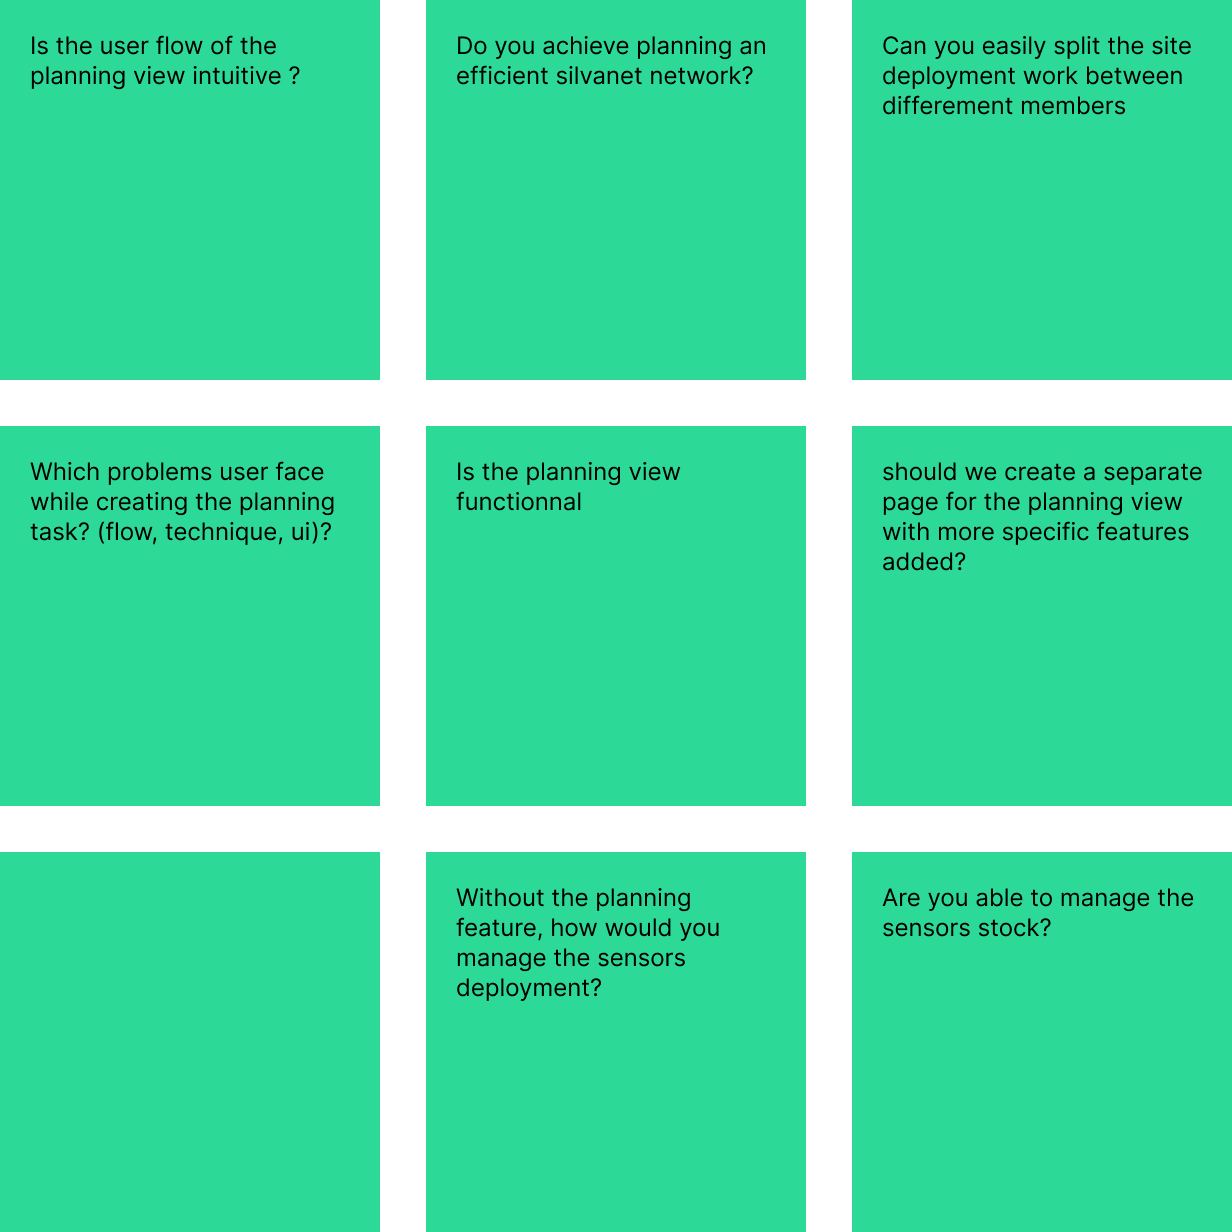
\includegraphics[width=10cm]{lotus_blossom_top}
  \caption{Ergebnis lotus blossom top}
  \label{fig:lotus_blossom_top}
\end{figure}
\begin{figure}[H]
  \centering
  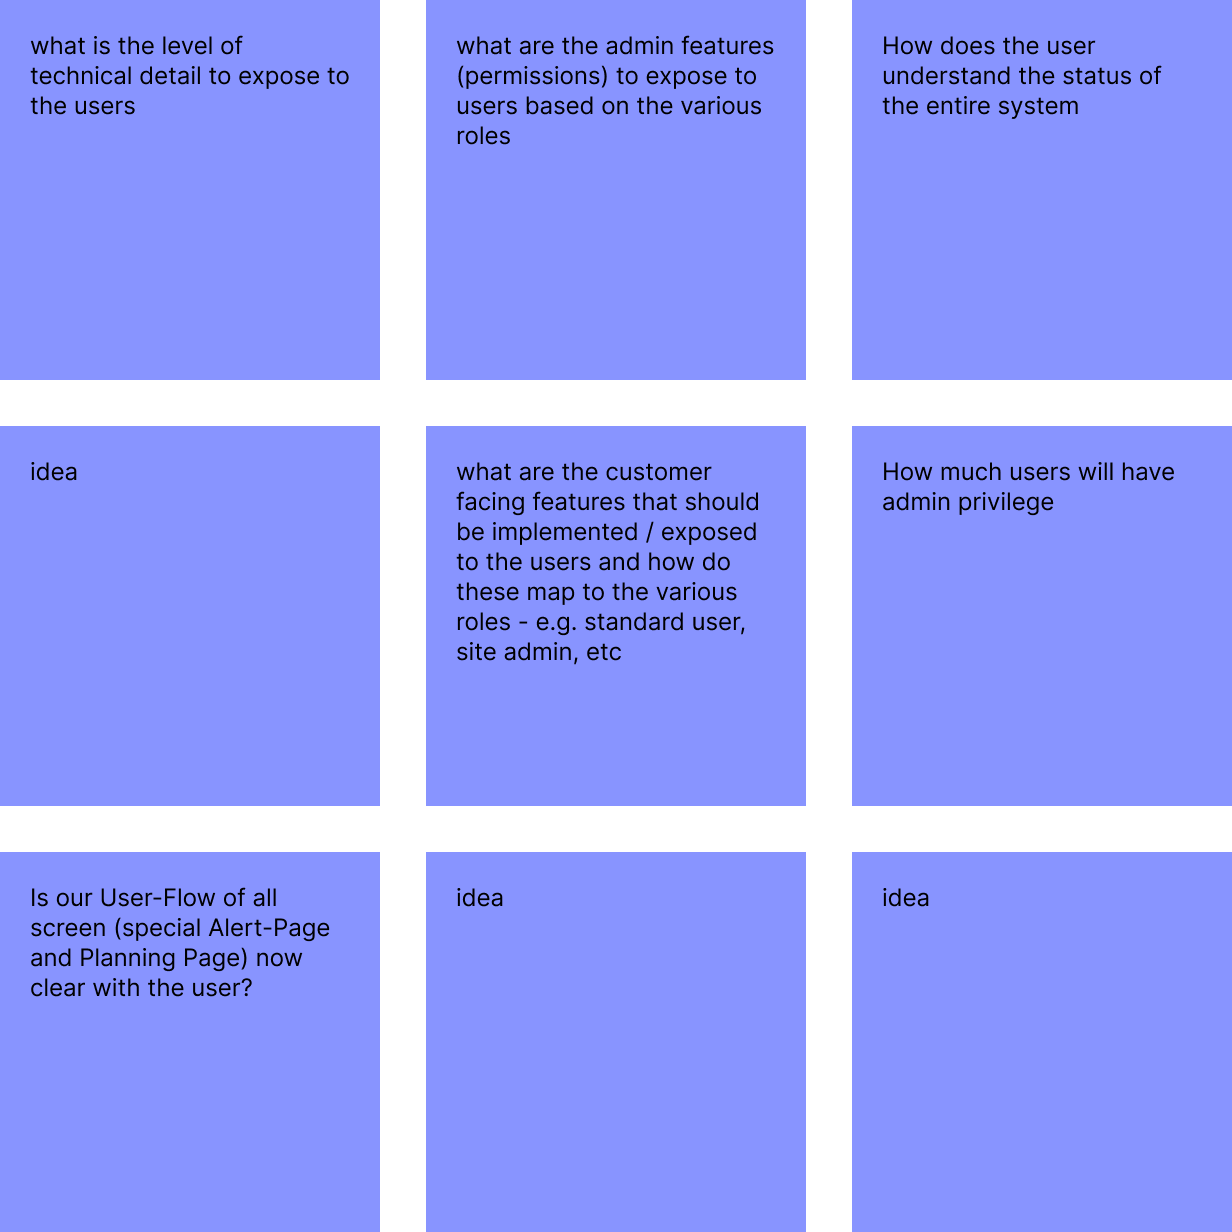
\includegraphics[width=10cm]{lotus_blossom_right}
  \caption{Ergebnis lotus blossom rechts}
  \label{fig:lotus_blossom_right}
\end{figure}
\begin{figure}[H]
  \centering
  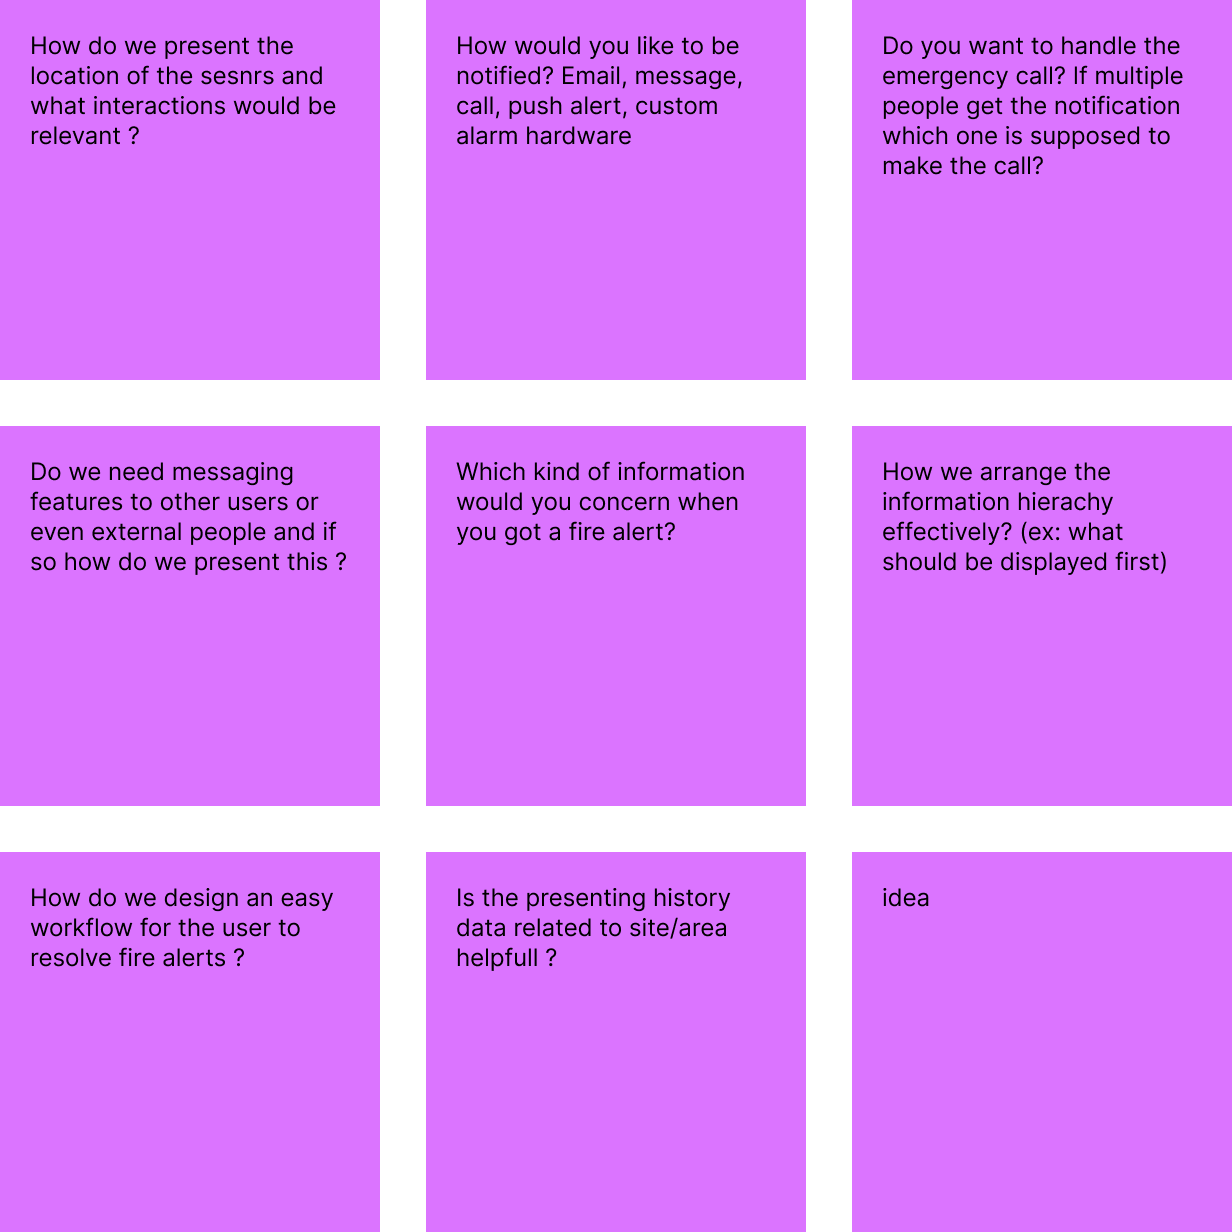
\includegraphics[width=10cm]{lotus_blossom_bottom_right}
  \caption{Ergebnis lotus blossom unten rechts}
  \label{fig:lotus_blossom_bottom_right}
\end{figure}
\begin{figure}[H]
  \centering
  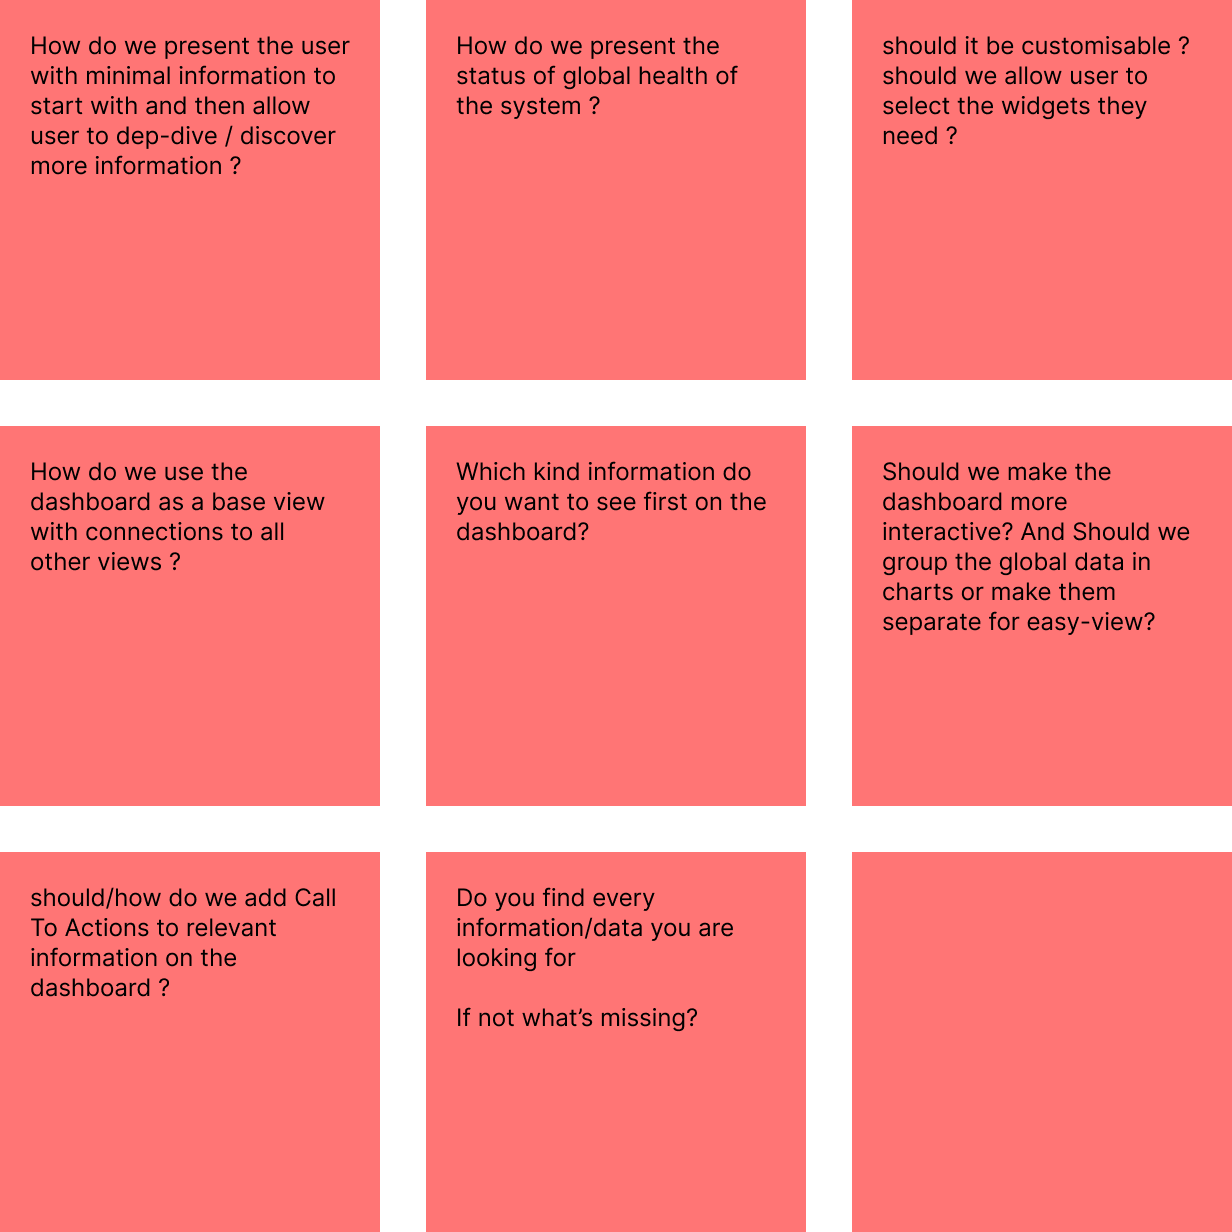
\includegraphics[width=10cm]{lotus_blossom_bottom}
  \caption{Ergebnis lotus blossom unten}
  \label{fig:lotus_blossom_bottom}
\end{figure}
\begin{figure}[H]
  \centering
  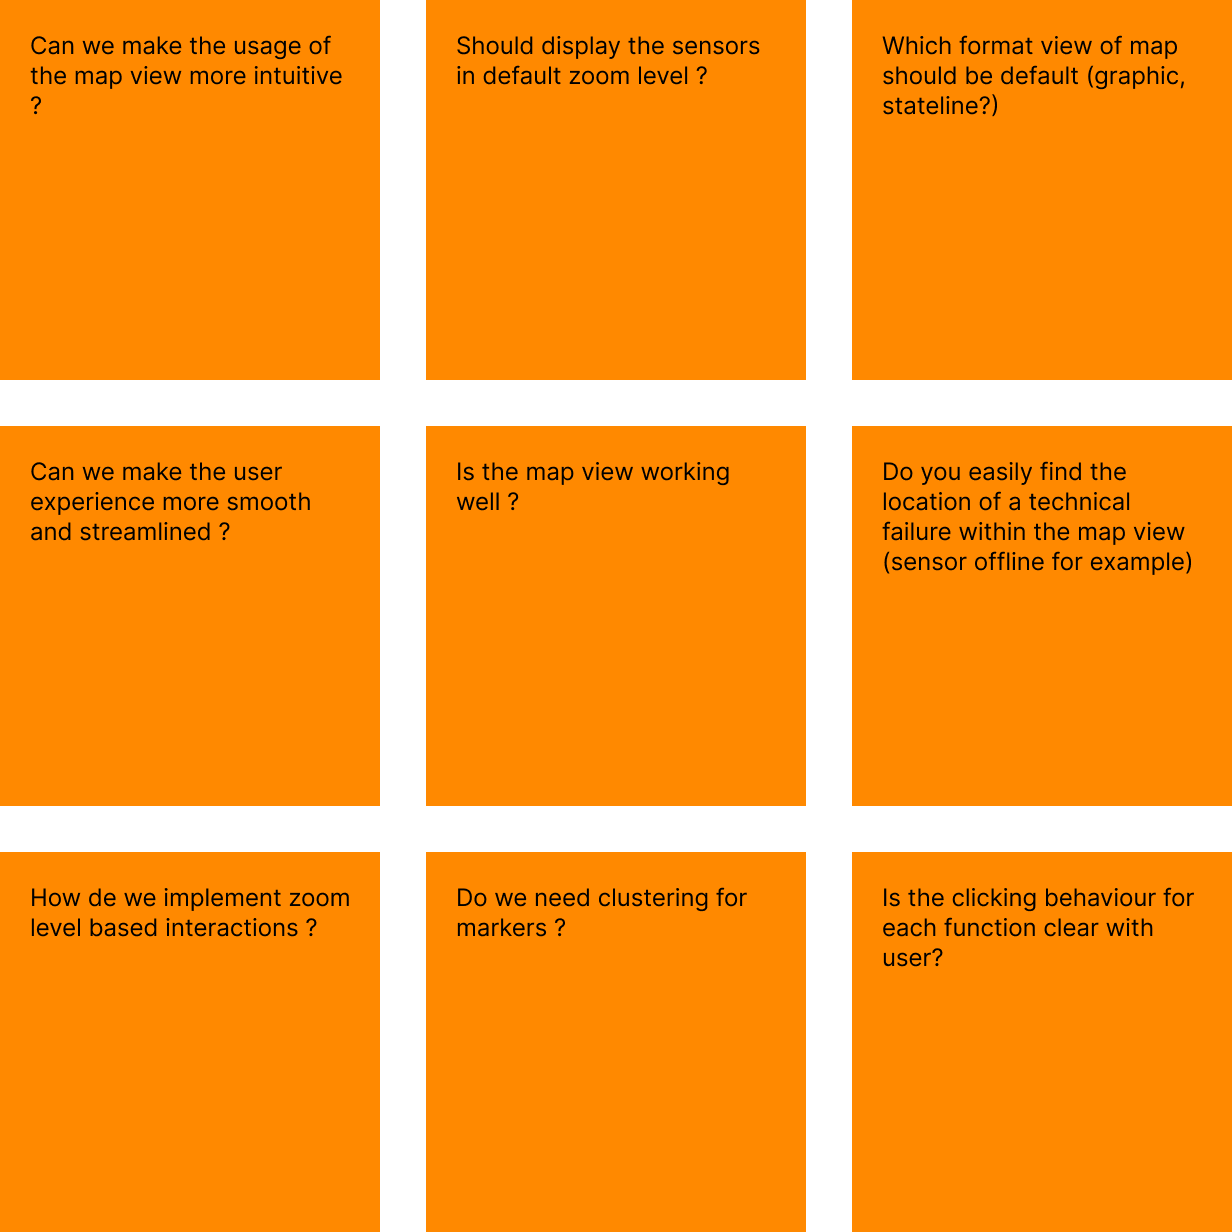
\includegraphics[width=10cm]{lotus_blossom_bottom_left}
  \caption{Ergebnis lotus blossom unten links}
  \label{fig:lotus_blossom_bottom_left}
\end{figure}
\begin{figure}[H]
  \centering
  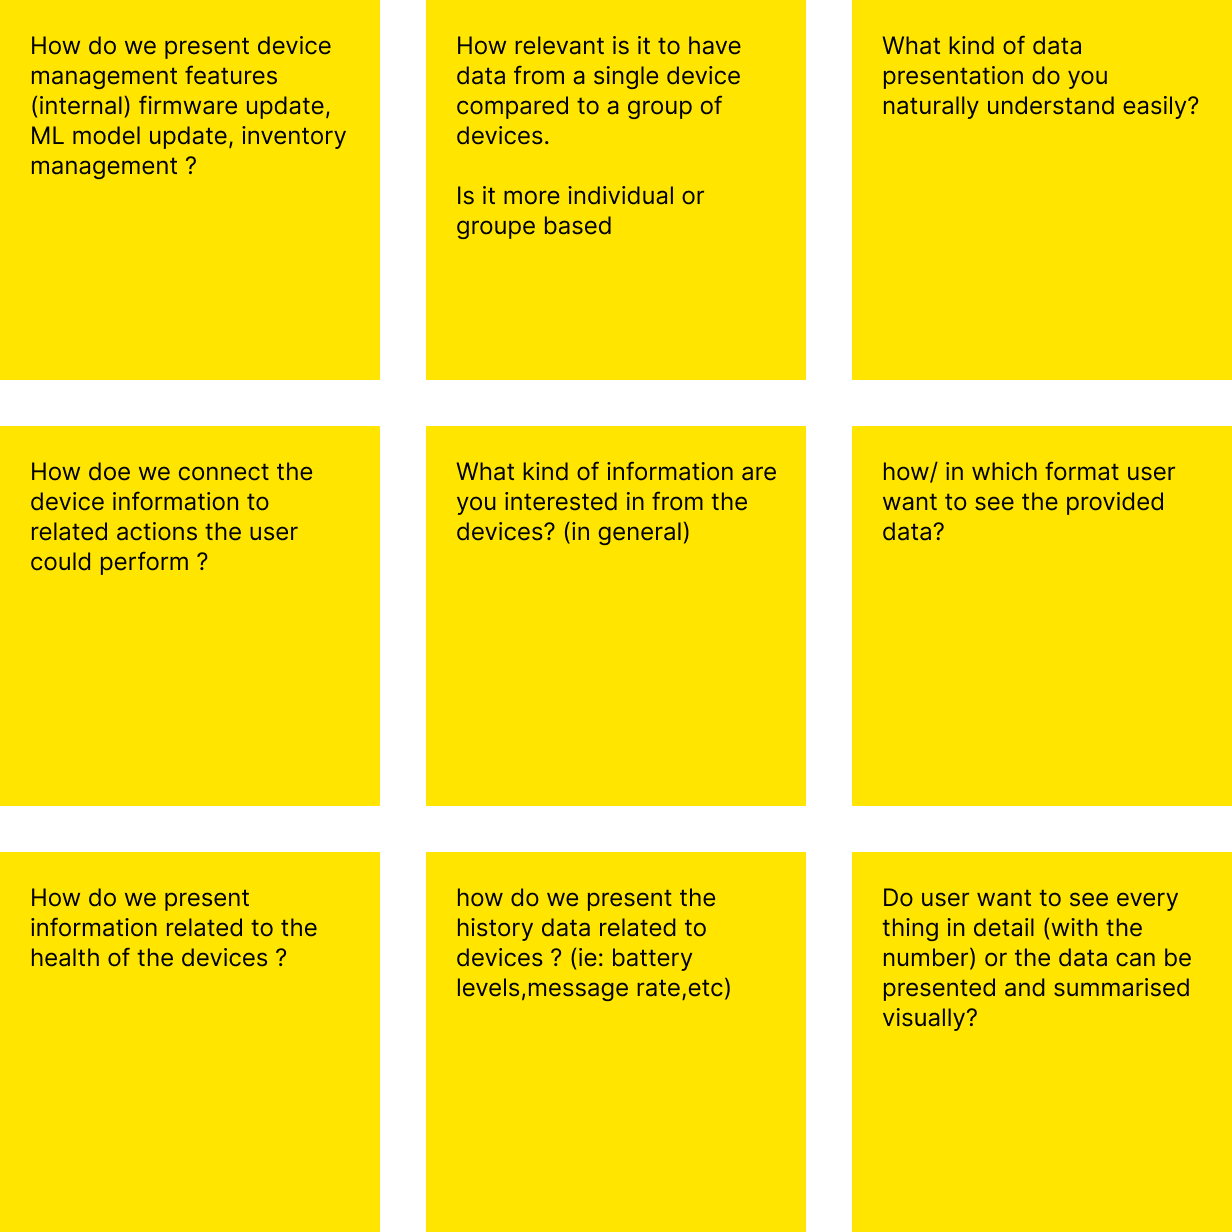
\includegraphics[width=10cm]{lotus_blossom_top_left}
  \caption{Ergebnis lotus blossom oben links}
  \label{fig:lotus_blossom_top_left}
\end{figure}
\section{Ergebnis der UX-Methode des Question Board, das von Dryads Cloud-Team mit dem Miro-Tool erstellt wurde} \label{appendix:question_board}

\begin{figure}[H]
  \centering
  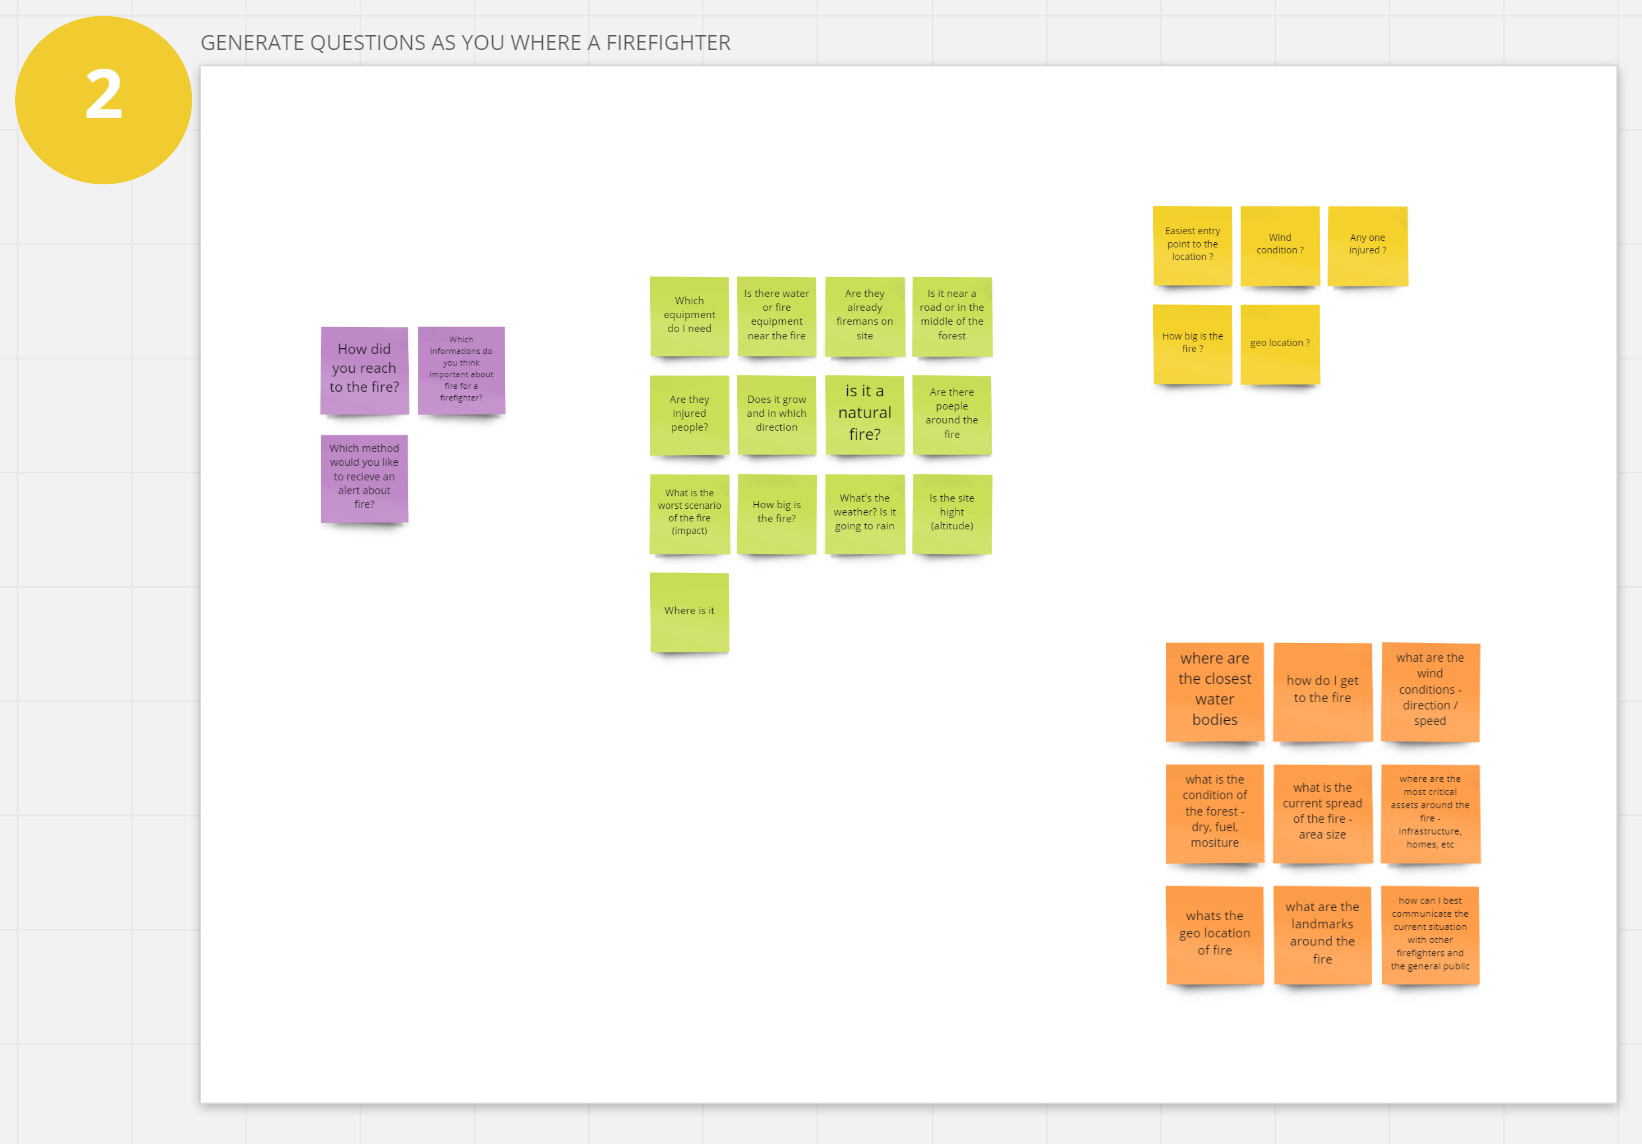
\includegraphics[width=\textwidth]{question_board_2}
  \caption{Question Board: Kollektive Generierung von Interogationen}
  \label{fig:question_board_2}
\end{figure}
\begin{figure}[H]
  \centering
  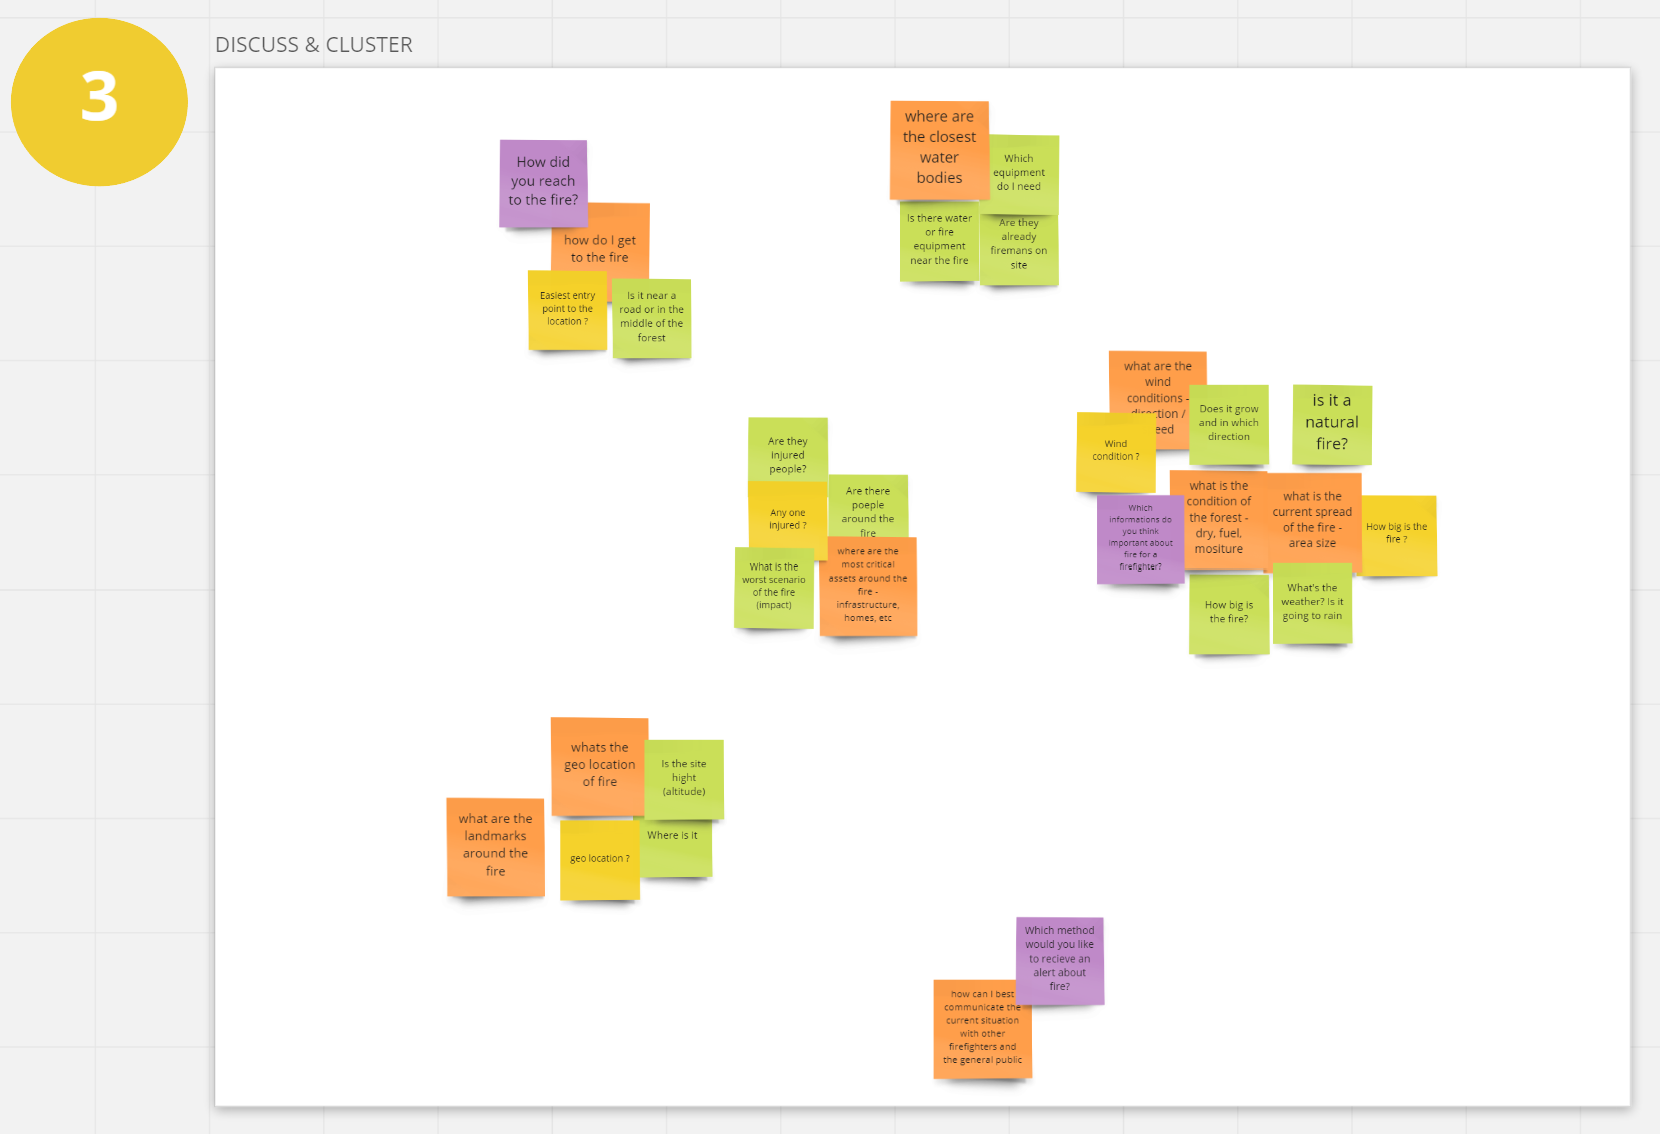
\includegraphics[width=\textwidth]{question_board_3}
  \caption{Question Board: Gruppierung von Interogationen zu gemeinsamen Themen}
  \label{fig:question_board_3}
\end{figure}
\begin{figure}[H]
  \centering
  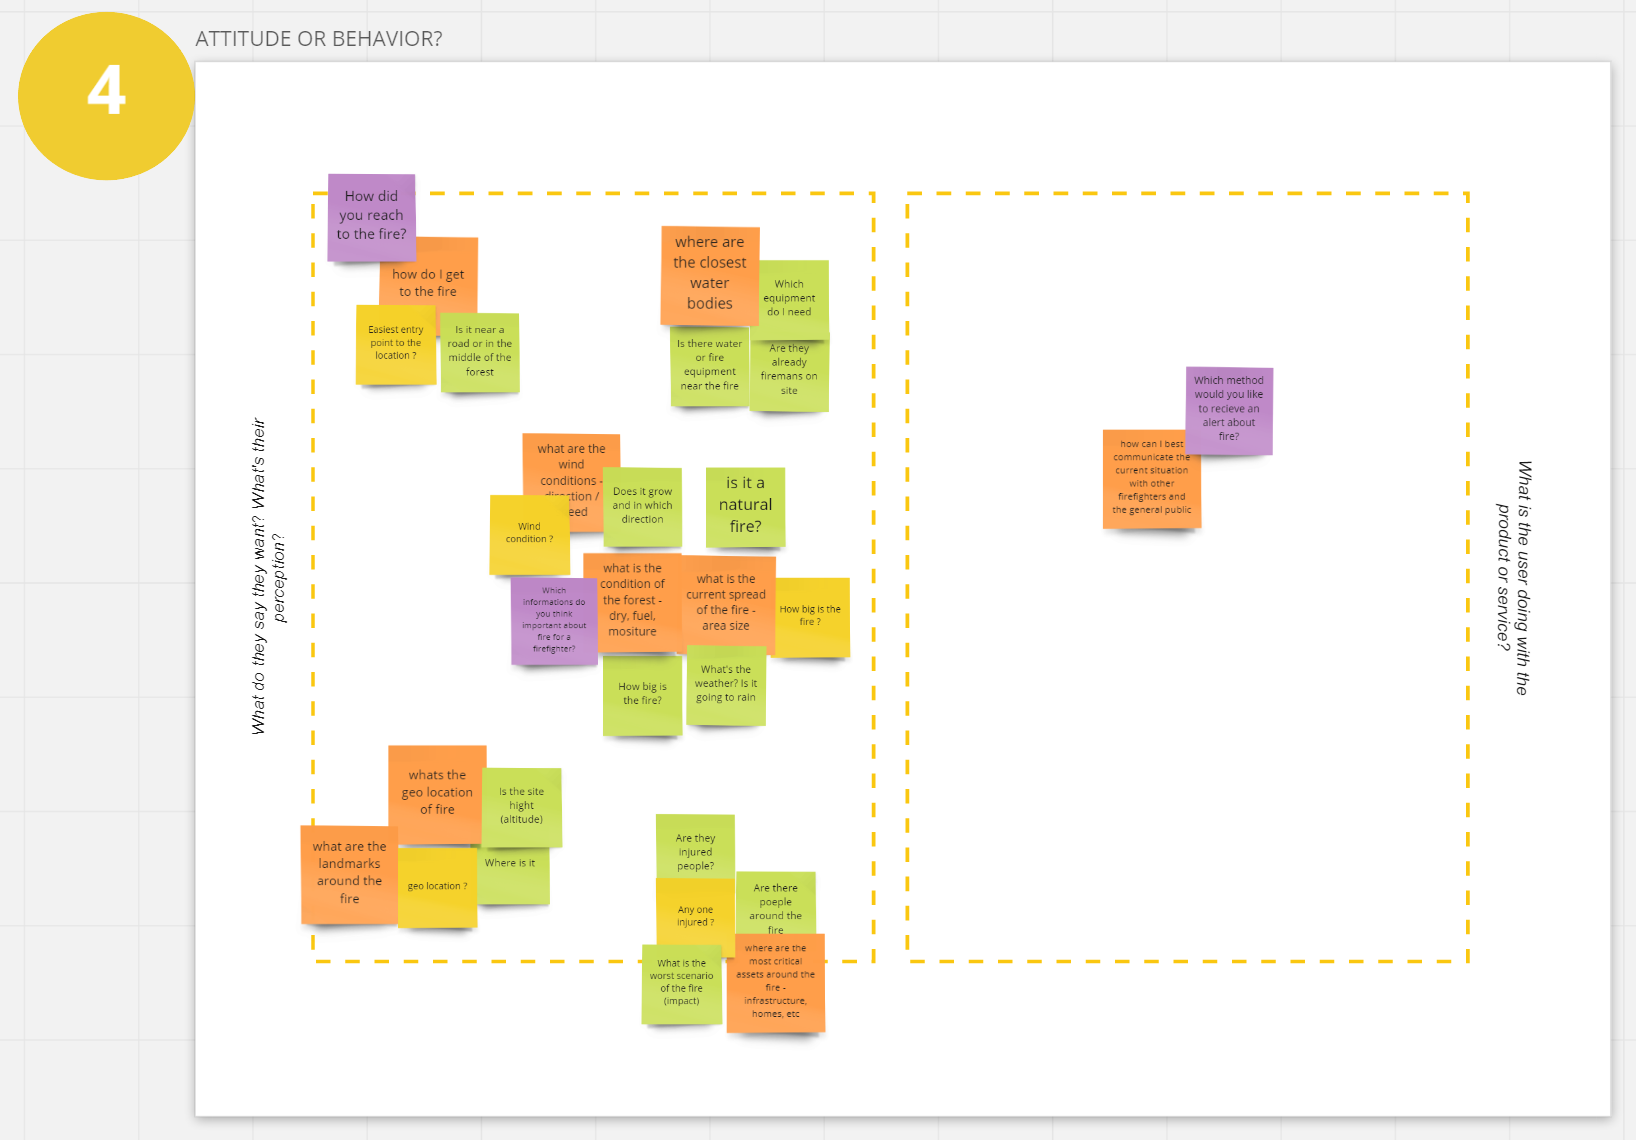
\includegraphics[width=\textwidth]{question_board_4}
  \caption{Question Board: Gruppierung der Probanden nach Interogation über Einstellung oder Verhalten}
  \label{fig:question_board_4}
\end{figure}
\begin{figure}[H]
  \centering
  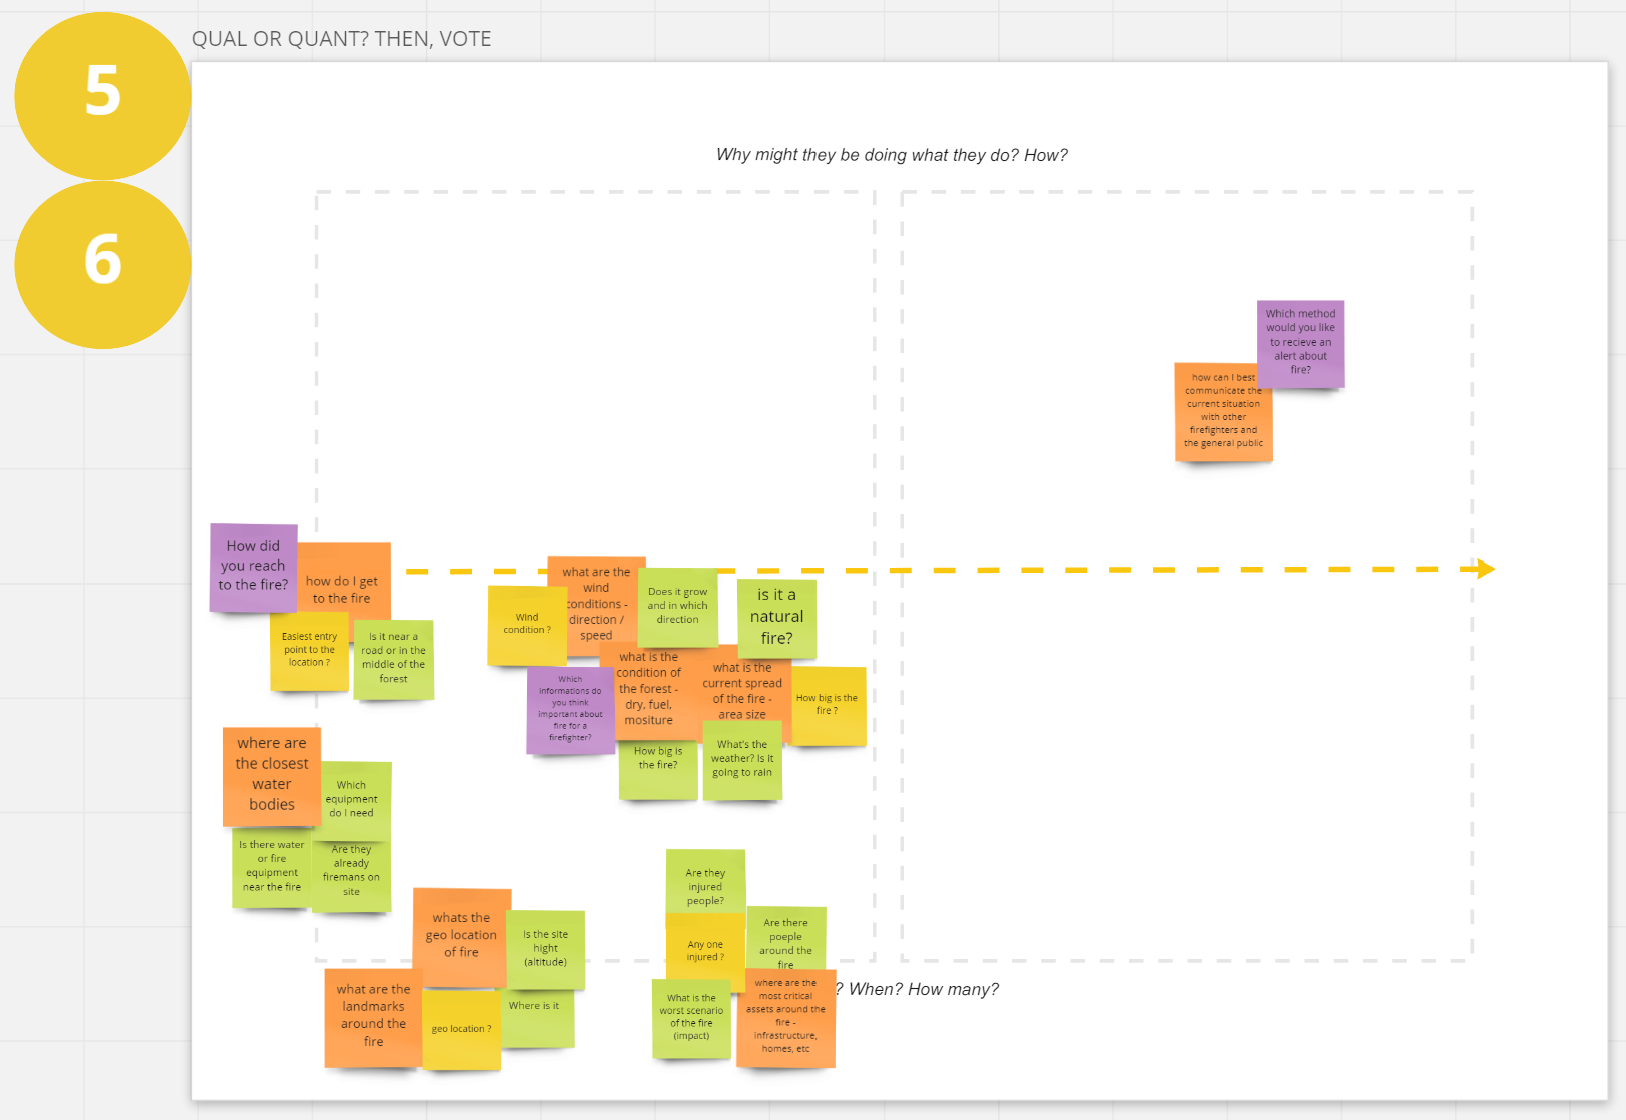
\includegraphics[width=\textwidth]{question_board_5}
  \caption{Question Board: Gruppierung der Themen nach Interogation über den quantitativen oder qualitativen Aspekt}
  \label{fig:question_board_5}
\end{figure}
\begin{figure}[H]
  \centering
  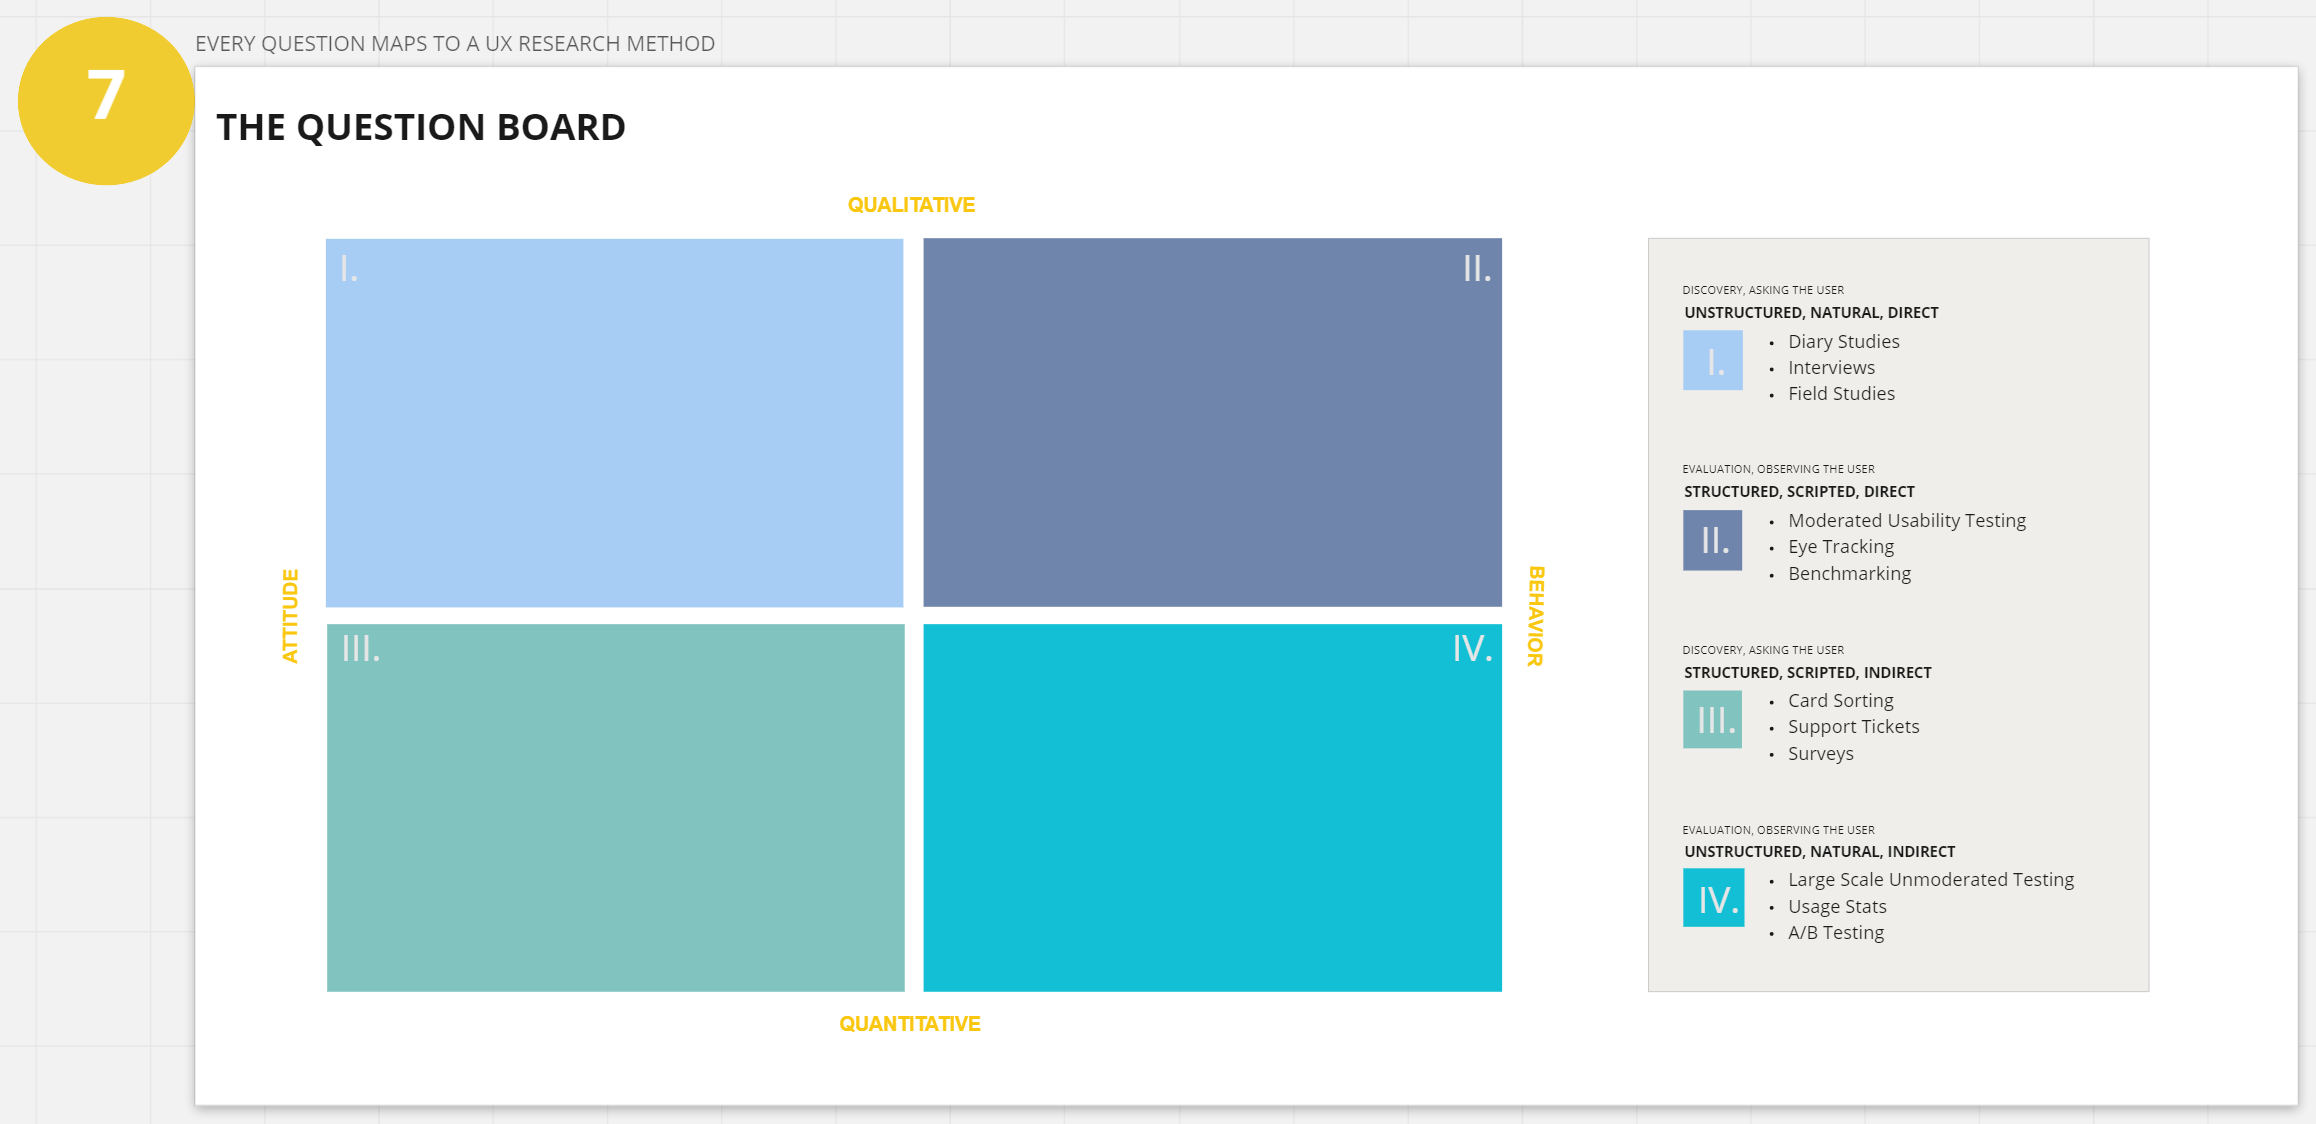
\includegraphics[width=\textwidth]{question_board_7}
  \caption{Question Board: Ansicht der möglichen Cluster mit ihrer zugehörigen Suchmethode}
  \label{fig:question_board_7}
\end{figure}

\section{Notizen aus der ergonomischen Inspektion der Webschnittstelle (Englisch)} \label{appendix:ergonomic-inspection}

\includepdf[
  pages=-,
  scale=0.75,
  pagecommand={\thispagestyle{plain}}
]{Statics/dryad-ergonomic-inspection.pdf}

\section{Formular für die Gemeinschaft der Feuerwehrleute (Deutsch)} \label{appendix:firefighter-survey}

\includepdf[
  pages=-,
  scale=0.75,
  pagecommand={\thispagestyle{plain}}
]{Statics/firefighter-survey-overview.pdf}

\section{Ergebnis der Auswertung der Antworten des Feuerwehrfragebogens (Englisch)} \label{appendix:firefighter_survey}

\begin{figure}[H]
  \centering
  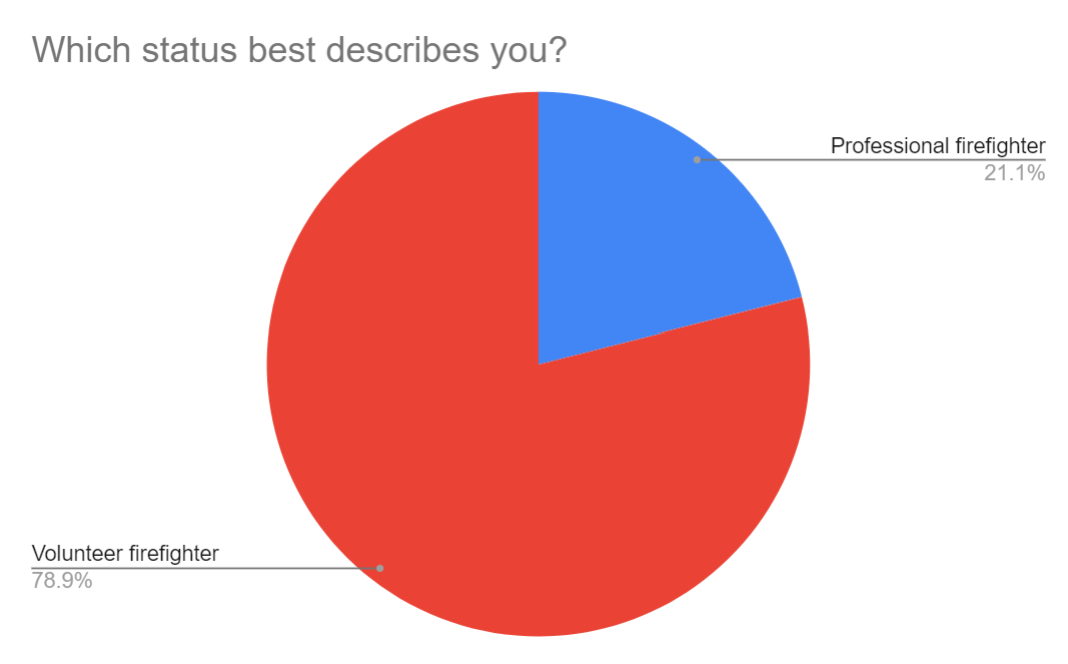
\includegraphics[width=11cm]{survey_graph_status}
  \caption{Verteilung des Berufsstatus}
  \label{fig:survey_graph_status}
\end{figure}

\begin{figure}[H]
  \centering
  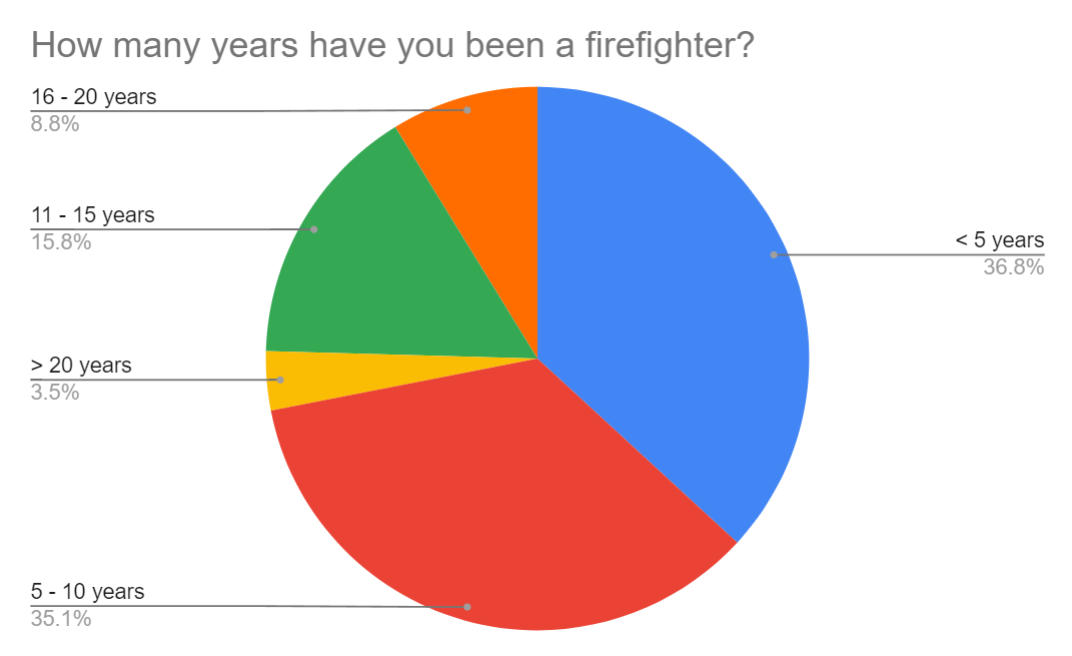
\includegraphics[width=11cm]{survey_graph_years}
  \caption{Verteilung der Dienstjahre}
  \label{fig:survey_graph_years}
\end{figure}

\begin{figure}[H]
  \centering
  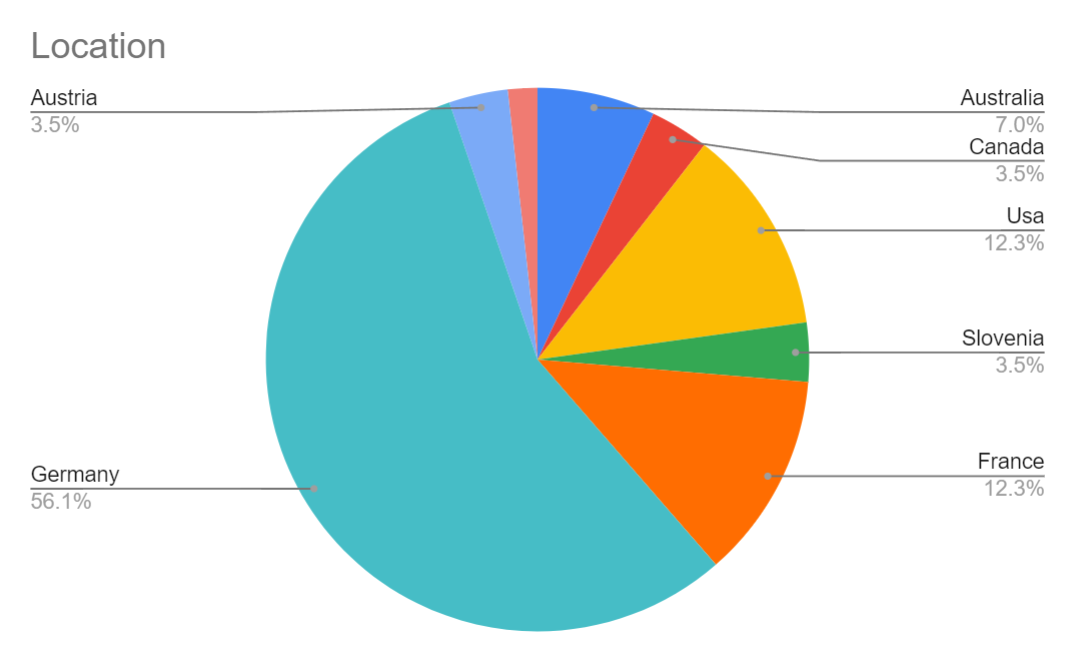
\includegraphics[width=11cm]{survey_graph_location}
  \caption{Geografische Verteilung der Antworten des Fragebogens}
  \label{fig:survey_graph_location}
\end{figure}

\begin{figure}[H]
  \centering
  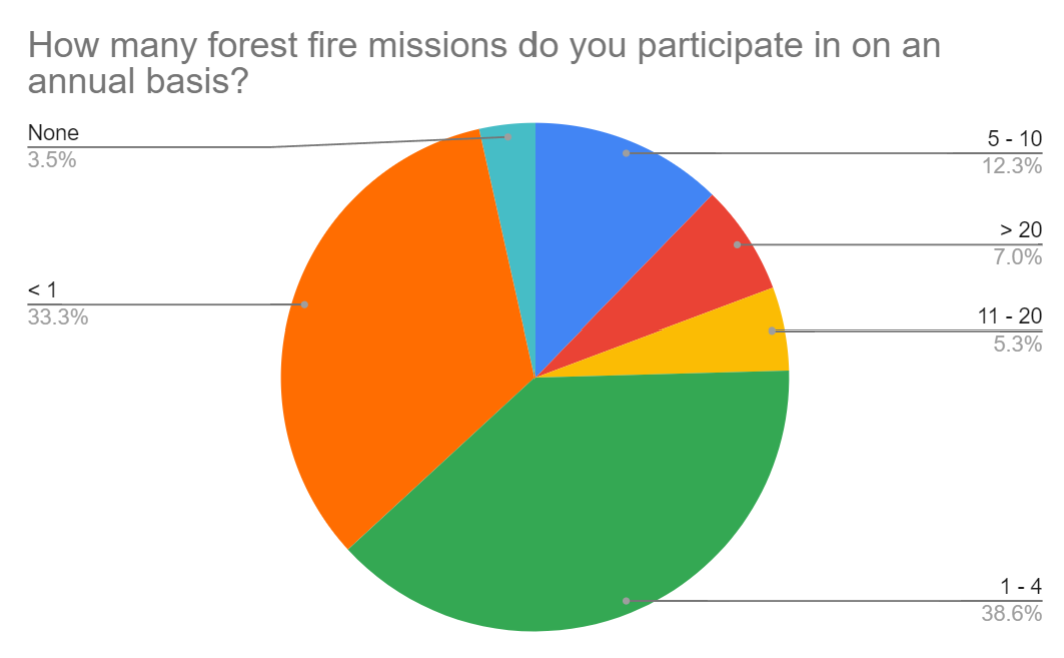
\includegraphics[width=11cm]{survey_graph_missions}
  \caption{Verteilung der durchschnittlich beteiligten Waldbrandeinsätze im Jahr}
  \label{fig:survey_graph_missions}
\end{figure}

\begin{figure}[H]
  \centering
  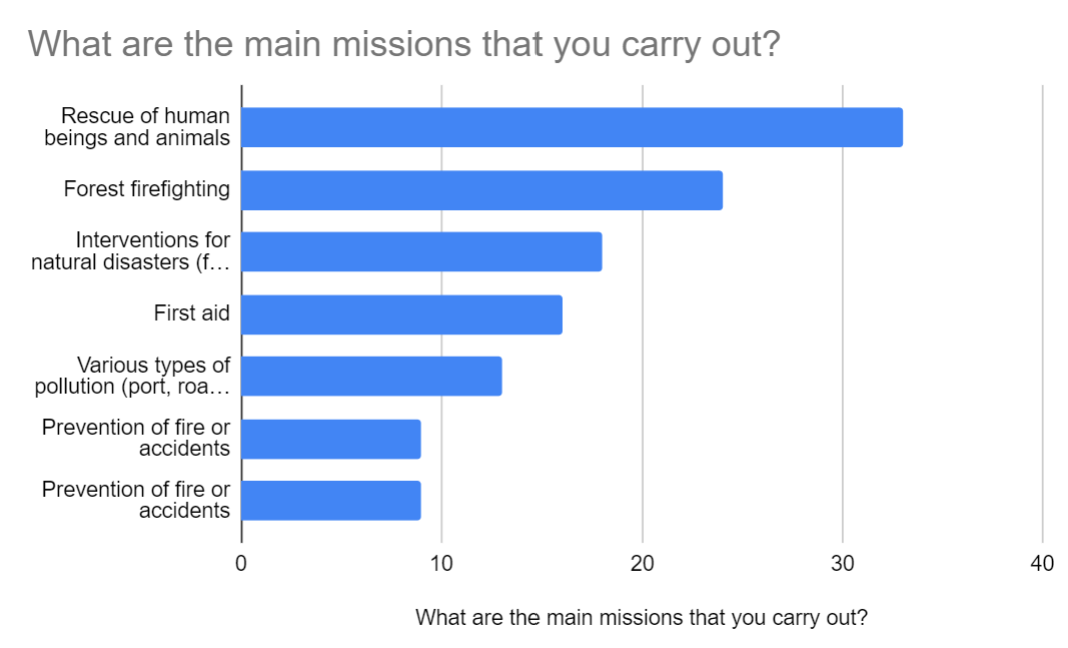
\includegraphics[width=11cm]{survey_graph_main_missions}
  \caption{Verteilung der verschiedenen Aufgaben, die hauptsächlich während des Dienstes erledigt werden}
  \label{fig:survey_graph_main_missions}
\end{figure}

\begin{figure}[H]
  \centering
  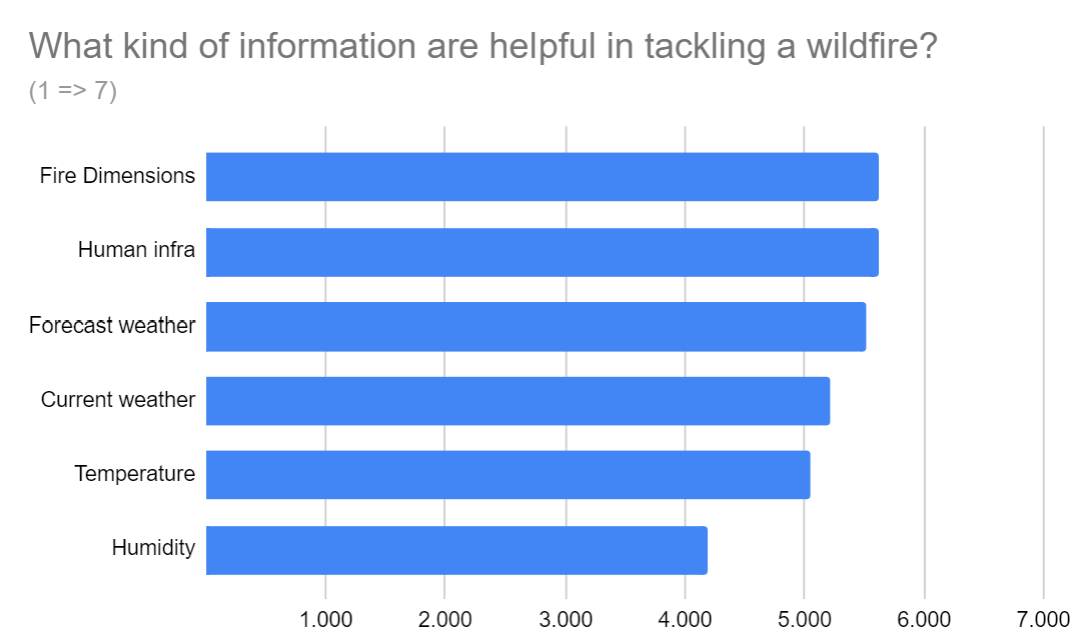
\includegraphics[width=11cm]{survey_graph_tackling}
  \caption{Relevanz der Daten zur Bekämpfung eines Waldbrandes}
  \label{fig:survey_graph_tackling}
\end{figure}

\begin{figure}[H]
  \centering
  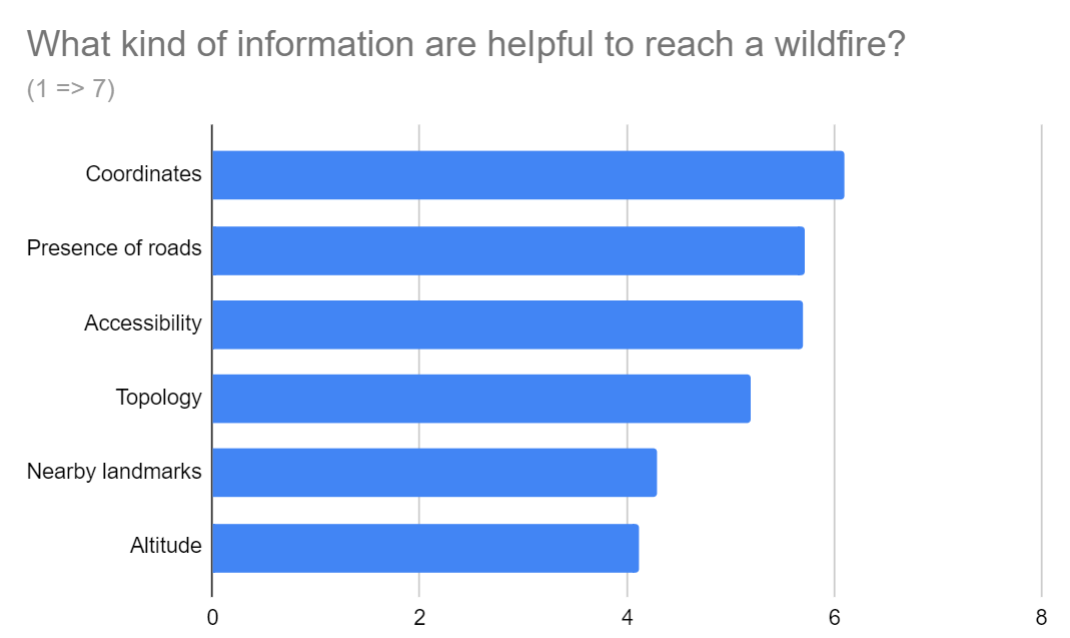
\includegraphics[width=11cm]{survey_graph_reach_fire}
  \caption{Relevanz der Daten, die den Zugang zu einem Waldbrand ermöglichen}
  \label{fig:survey_graph_reach_fire}
\end{figure}

\begin{figure}[H]
  \centering
  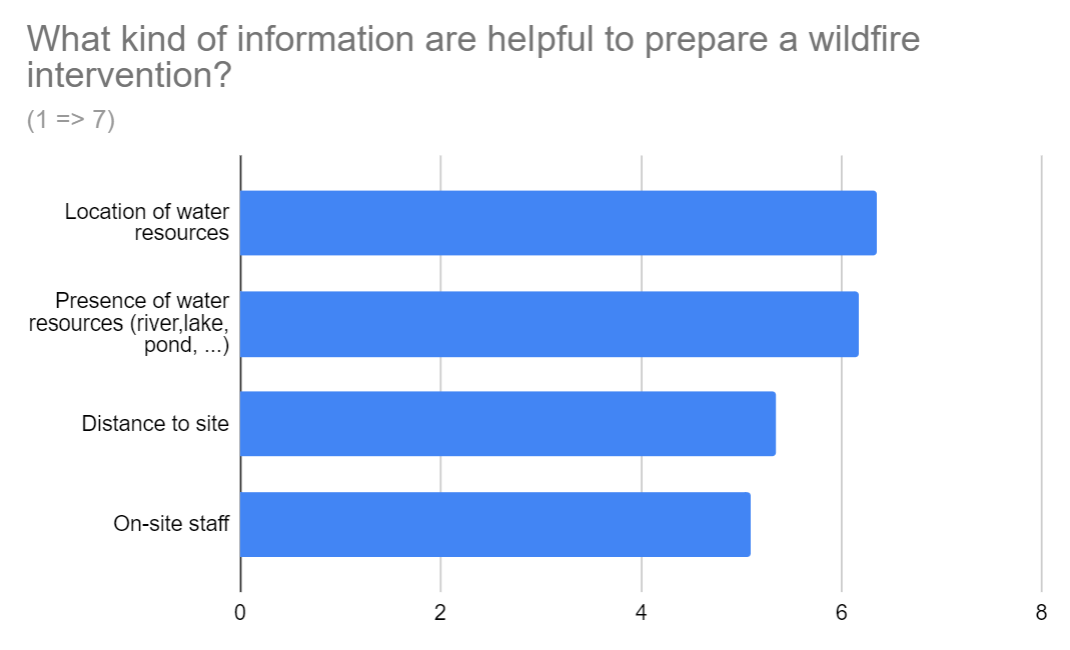
\includegraphics[width=11cm]{survey_graph_prepare}
  \caption{Relevanz der Daten zur Vorbereitung eines Feuerwehreinsatzes}
  \label{fig:survey_graph_prepare}
\end{figure}

\begin{figure}[H]
  \centering
  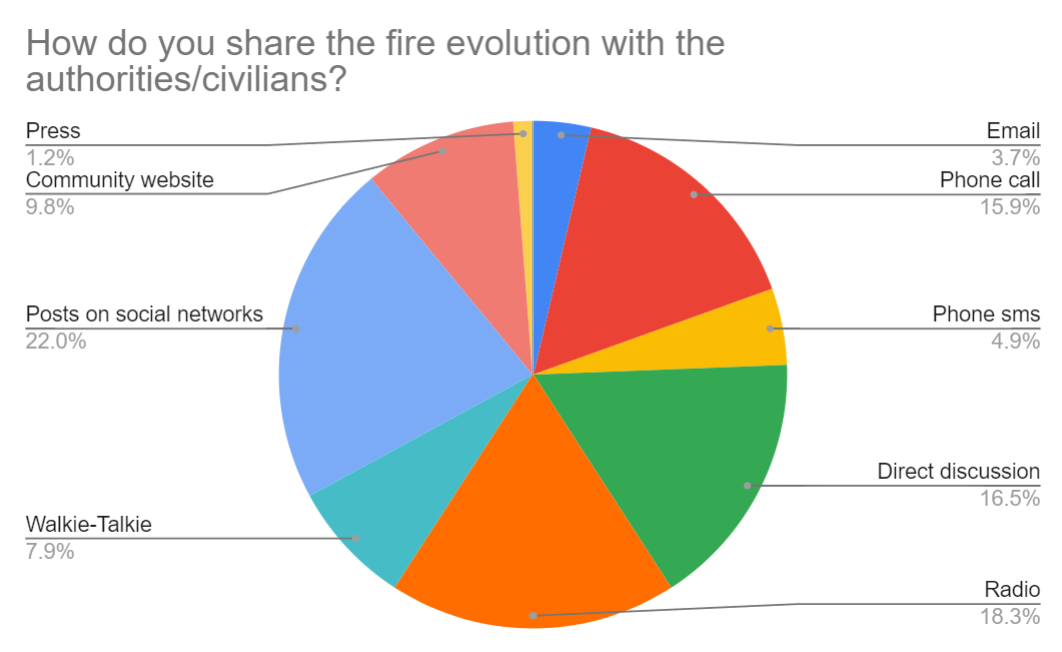
\includegraphics[width=11cm]{survey_graph_share_evolution}
  \caption{Verteilung der Methoden, die verwendet werden, um die Entwicklung eines Waldbrandes mitzuteilen}
  \label{fig:survey_graph_share_evolution}
\end{figure}

\begin{figure}[H]
  \centering
  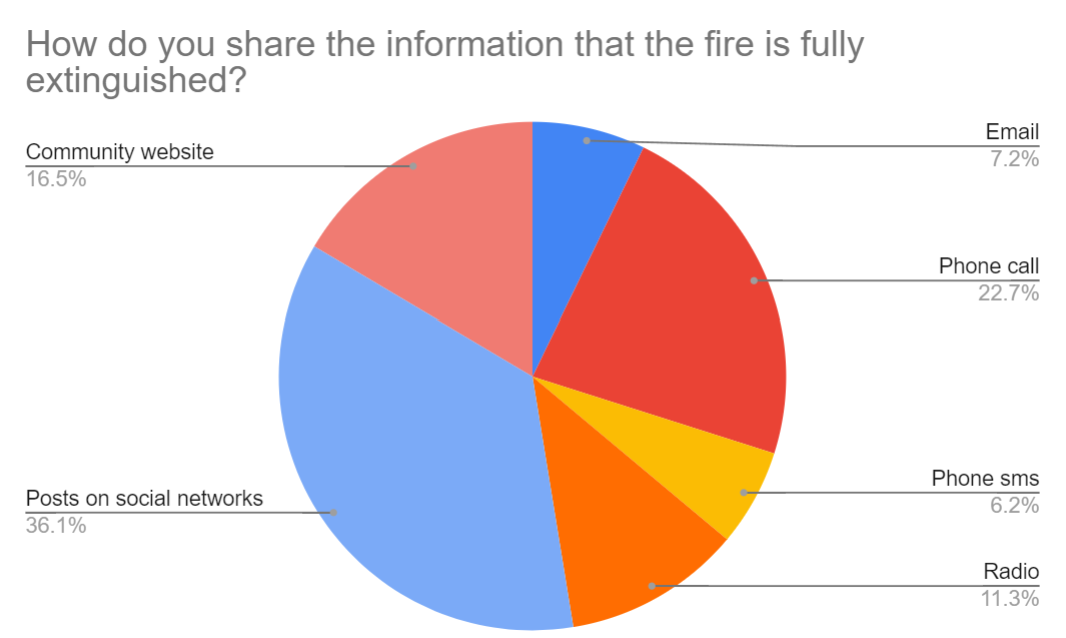
\includegraphics[width=11cm]{survey_graph_share_extinction}
  \caption{Verteilung der Methoden, mit denen die Nachricht vom Löschen eines Waldbrandes geteilt wird}
  \label{fig:survey_graph_share_extinction}
\end{figure}

\begin{figure}[H]
  \centering
  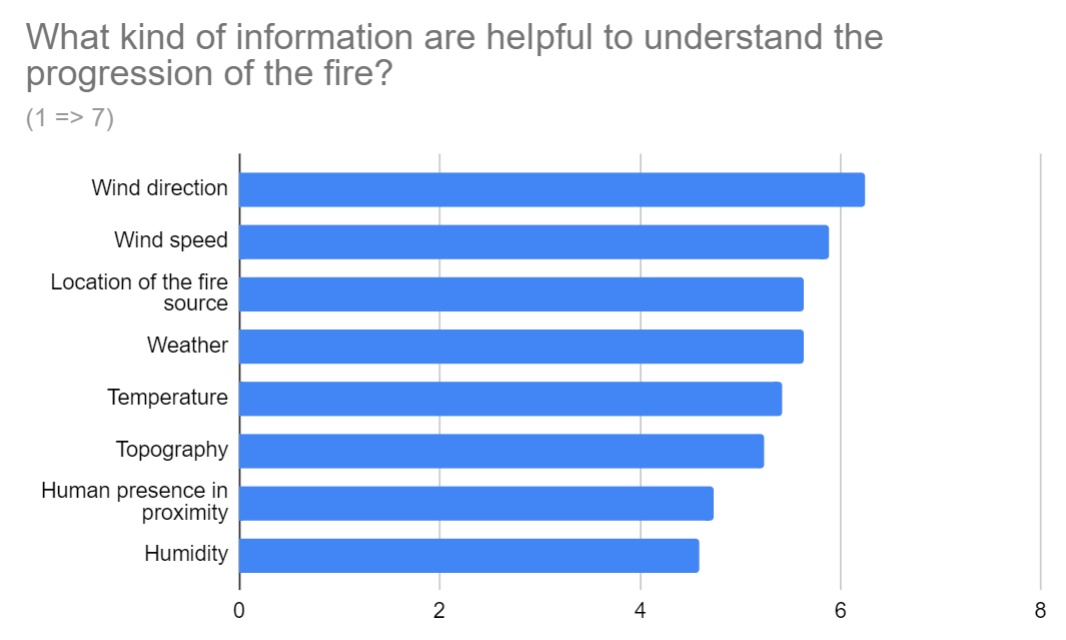
\includegraphics[width=11cm]{survey_graph_progression}
  \caption{Relevanz der Daten zum Verständnis der Entwicklung eines Waldbrands}
  \label{fig:survey_graph_progression}
\end{figure}

\begin{figure}[H]
  \centering
  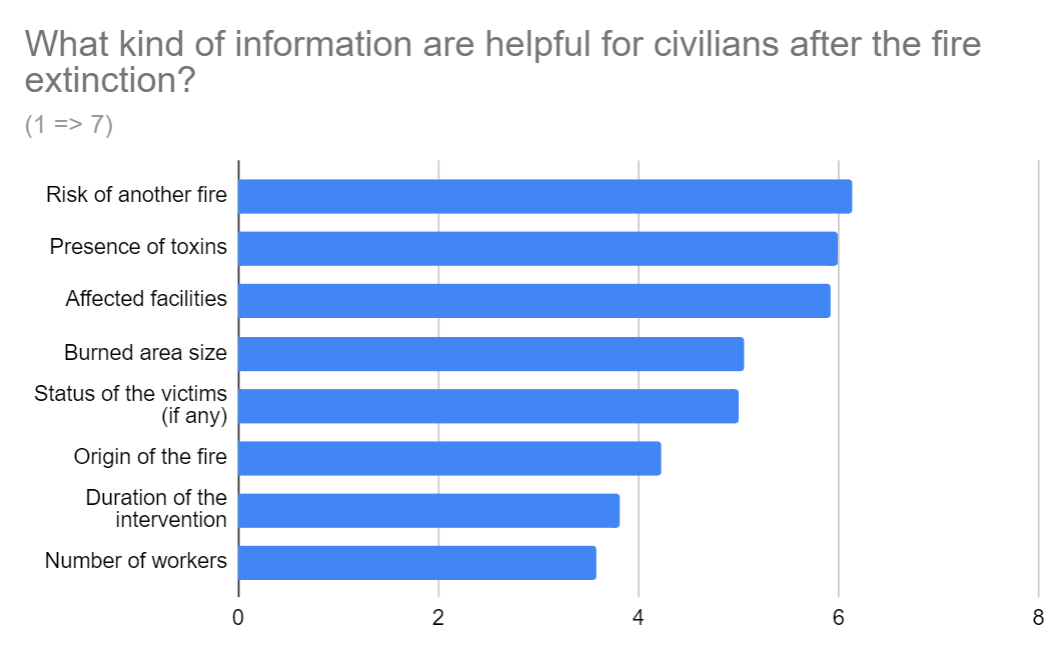
\includegraphics[width=11cm]{survey_graph_infos_civilians}
  \caption{Relevanz der Daten, die nach dem Löschen eines Waldbrandes mit Zivilisten geteilt werden sollen}
  \label{fig:survey_graph_infos_civilians}
\end{figure}

\begin{figure}[H]
  \centering
  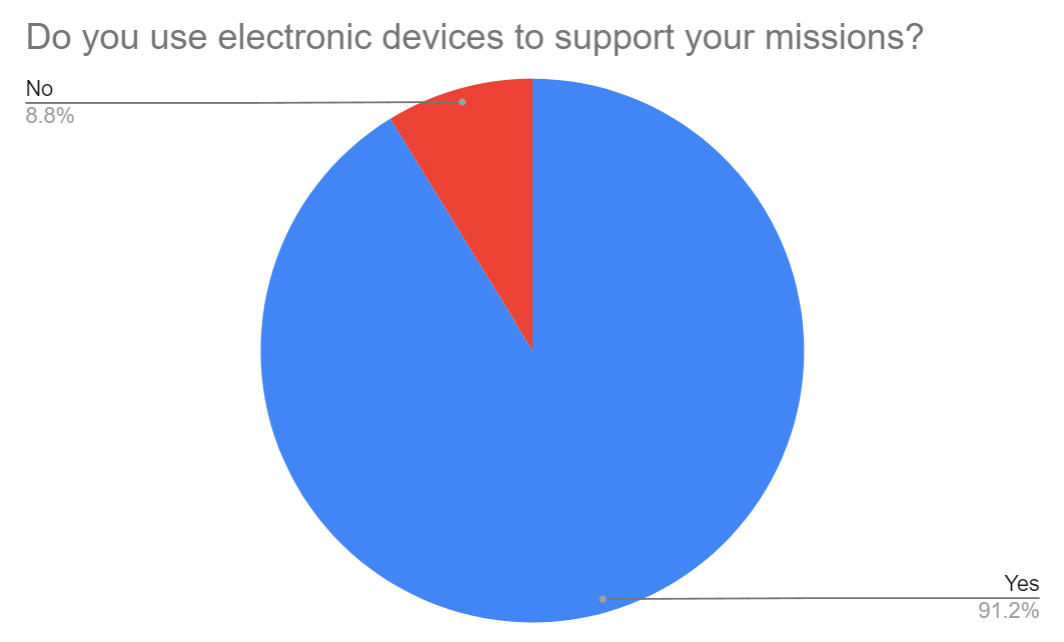
\includegraphics[width=11cm]{survey_graph_use_devices}
  \caption{Verteilung der Feuerwehrleute, die elektronische Geräte zur Unterstützung ihrer Arbeit verwenden}
  \label{fig:survey_graph_use_devices}
\end{figure}

\begin{figure}[H]
  \centering
  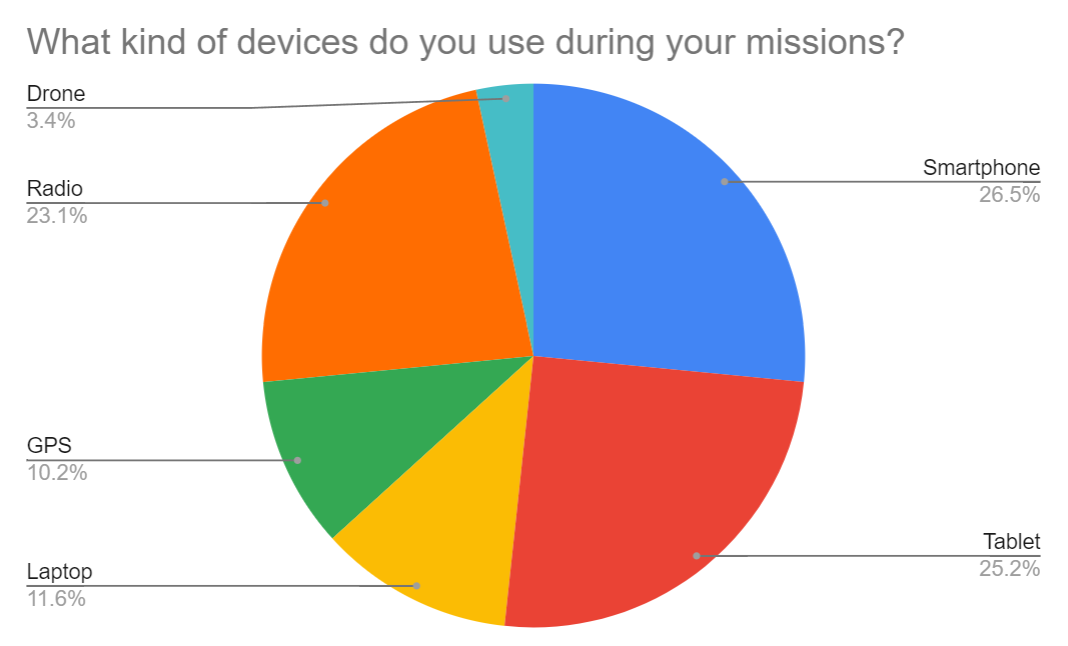
\includegraphics[width=11cm]{survey_graph_devices_mission}
  \caption{Verteilung der Arten von Elektrogeräten, die bei den Missionen verwendet wurden}
  \label{fig:survey_graph_devices_mission}
\end{figure}

\begin{figure}[H]
  \centering
  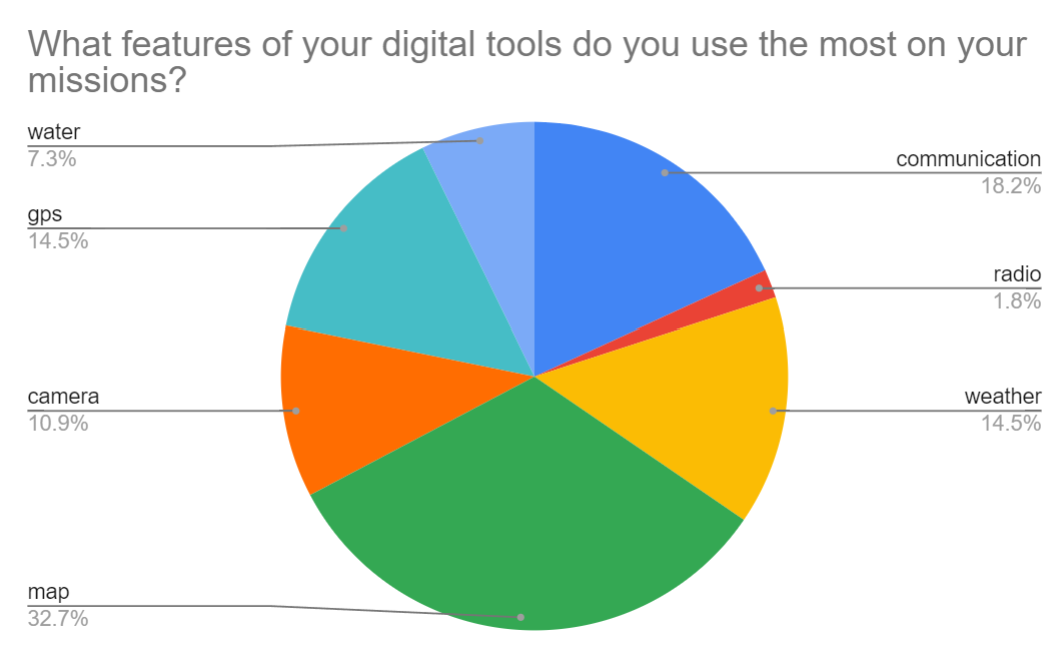
\includegraphics[width=11cm]{survey_graph_device_features}
  \caption{Verteilung der Funktionalität, die während der Missionen elektronische Geräte benutzte}
  \label{fig:survey_graph_device_features}
\end{figure}

\begin{figure}[H]
  \centering
  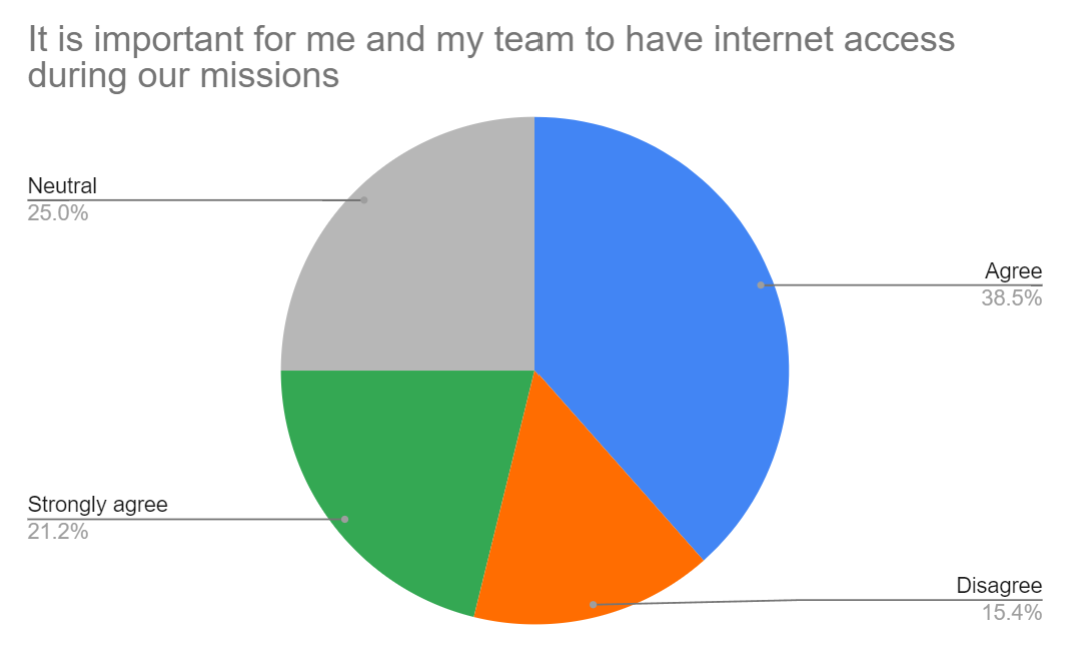
\includegraphics[width=11cm]{survey_graph_internet_missions}
  \caption{Verteilung der Internetnutzung während der Missionen}
  \label{fig:survey_graph_internet_missions}
\end{figure}

\begin{figure}[H]
  \centering
  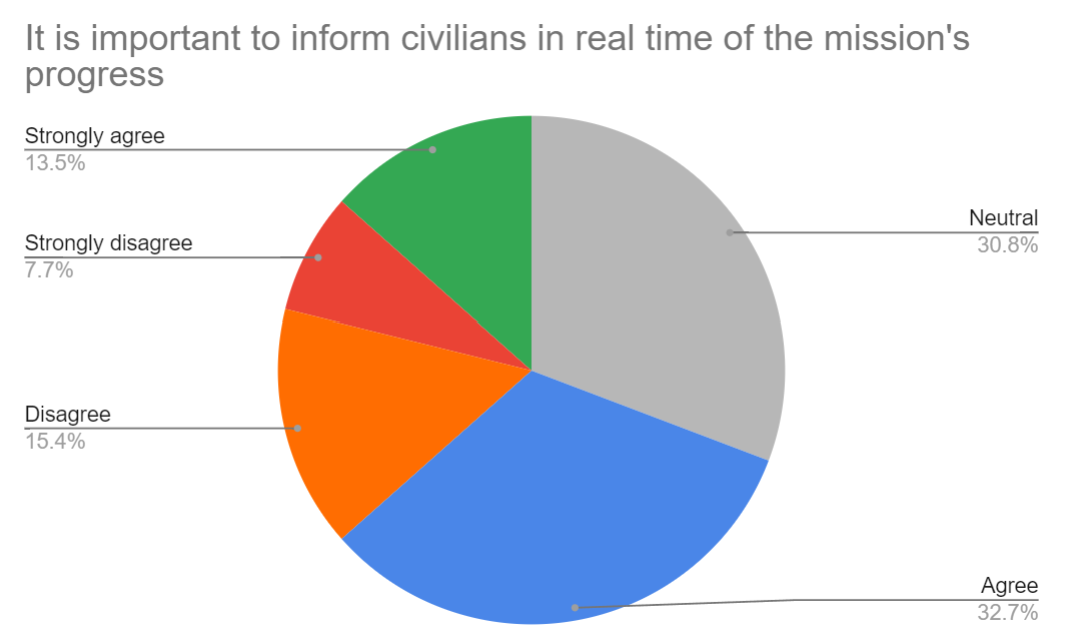
\includegraphics[width=11cm]{survey_graph_informcivilians}
  \caption{Relevanz der Information der Zivilbevölkerung über den Fortschritt der Mission zur Bekämpfung eines Waldbrandes}
  \label{fig:survey_graph_informcivilians}
\end{figure}

\begin{figure}[H]
  \centering
  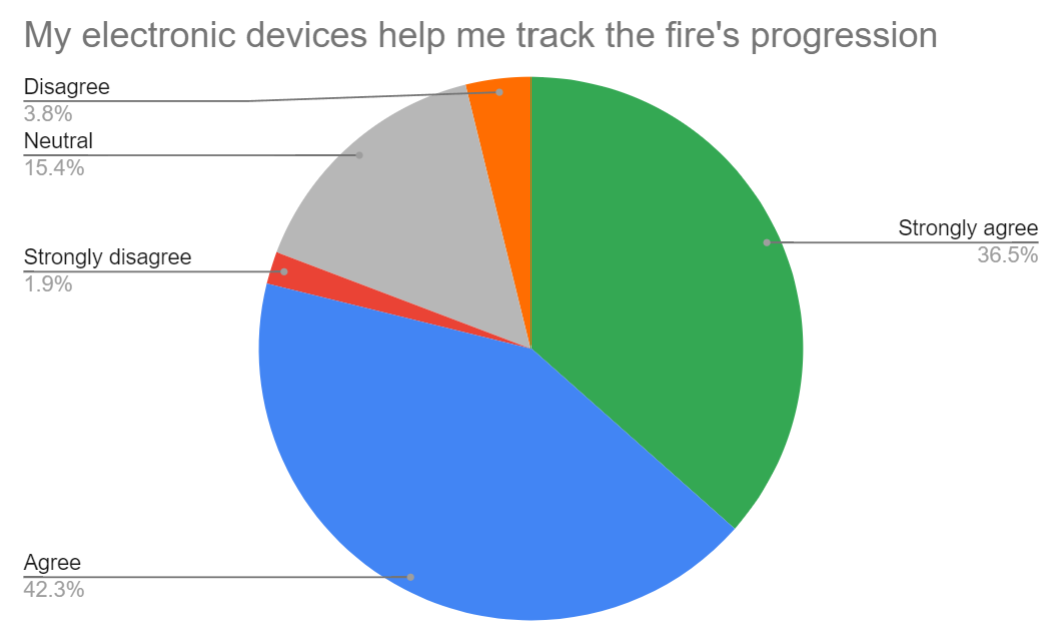
\includegraphics[width=11cm]{survey_graph_devices_helpfull}
  \caption{Relevanz von elektronischen Geräten für die Unterstützung bei der Überwachung der Ausbreitung eines Waldbrandes}
  \label{fig:survey_graph_devices_helpfull}
\end{figure}

\section{Ergebnisse einer Brainstorming-Sitzung zu den Features der interaktiven Karte, das von Dryads Cloud-Team mit dem Miro-Tool erstellt wurde} \label{appendix:question_board_map}

\begin{figure}[H]
  \centering
  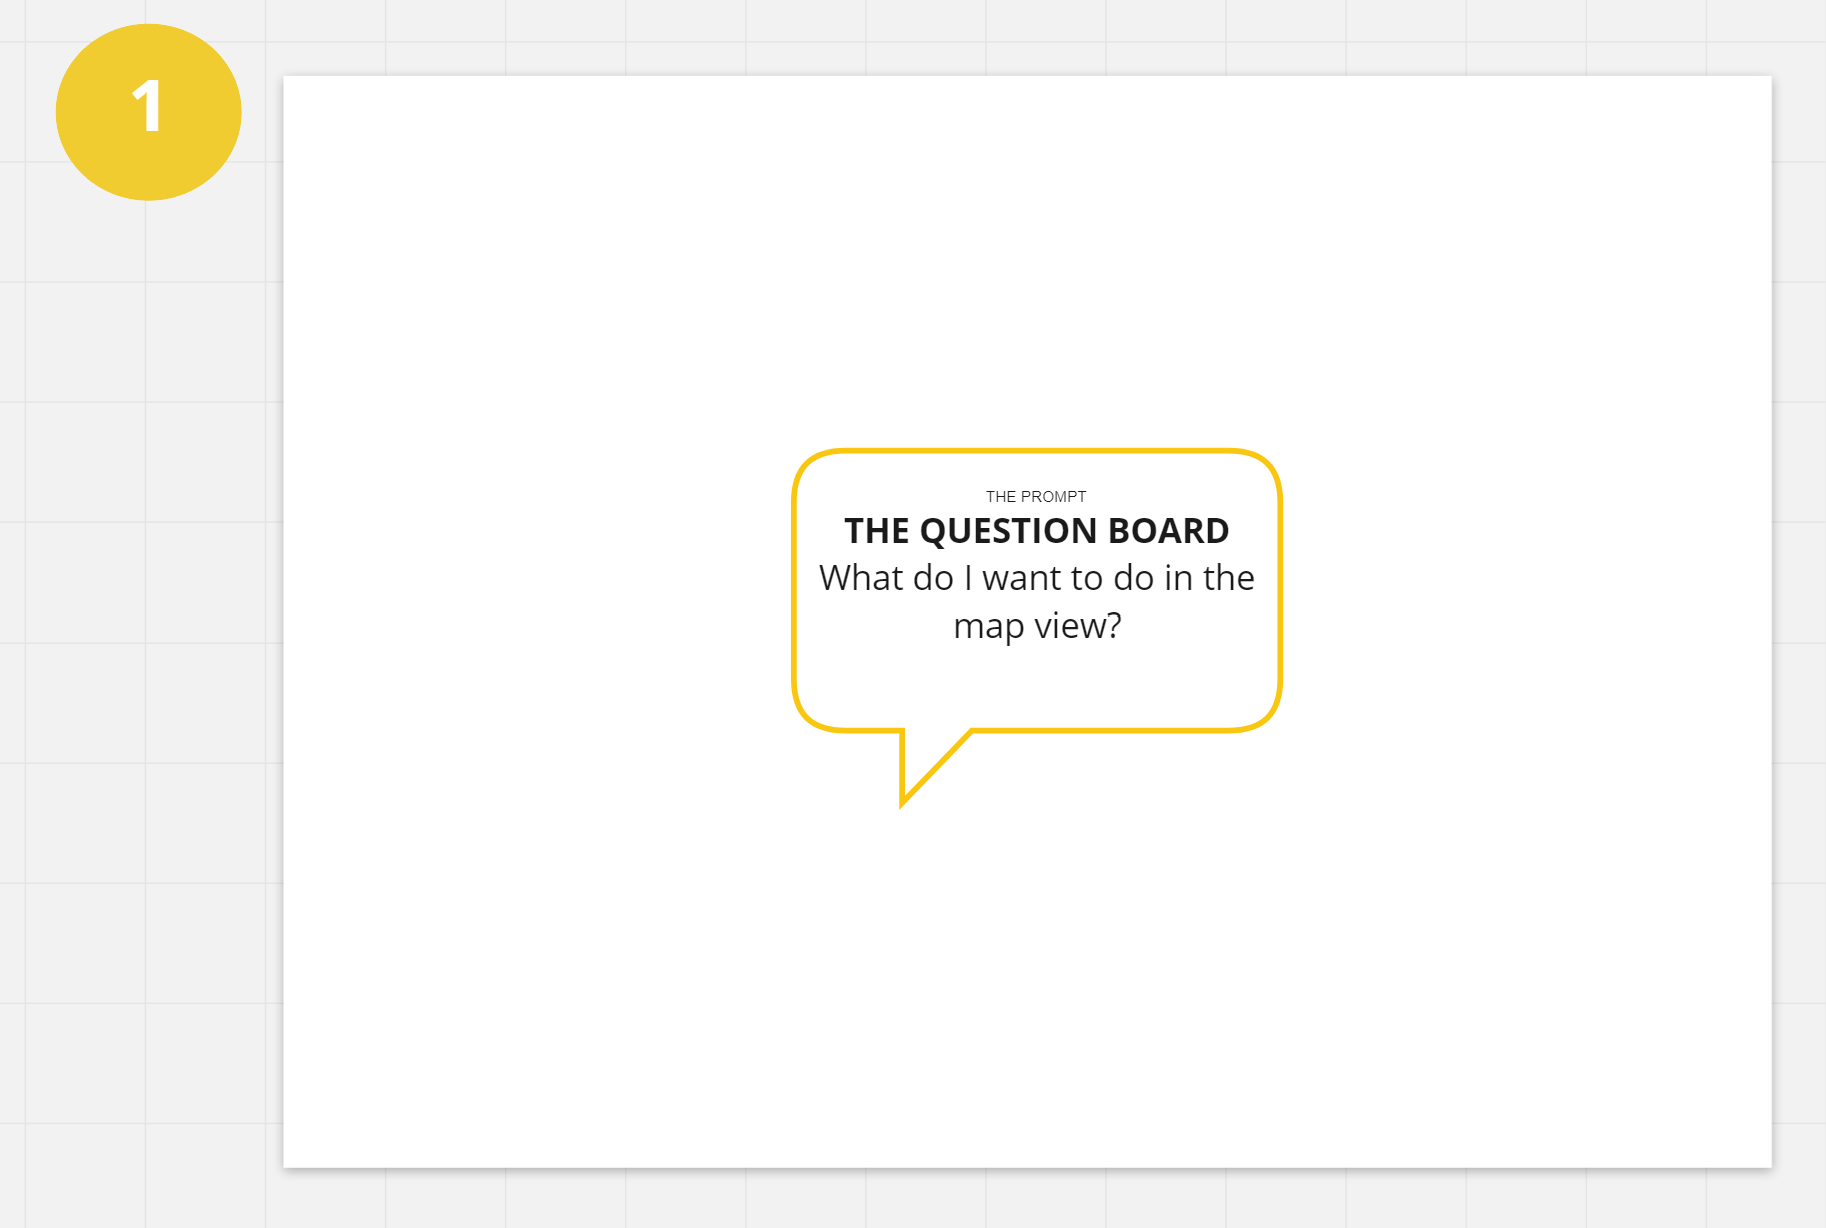
\includegraphics[width=\textwidth]{question_board_map_1}
  \caption{Präsentation des Question Board zur interaktiven Karte}
  \label{fig:question_board_map_1}
\end{figure}
\begin{figure}[H]
  \centering
  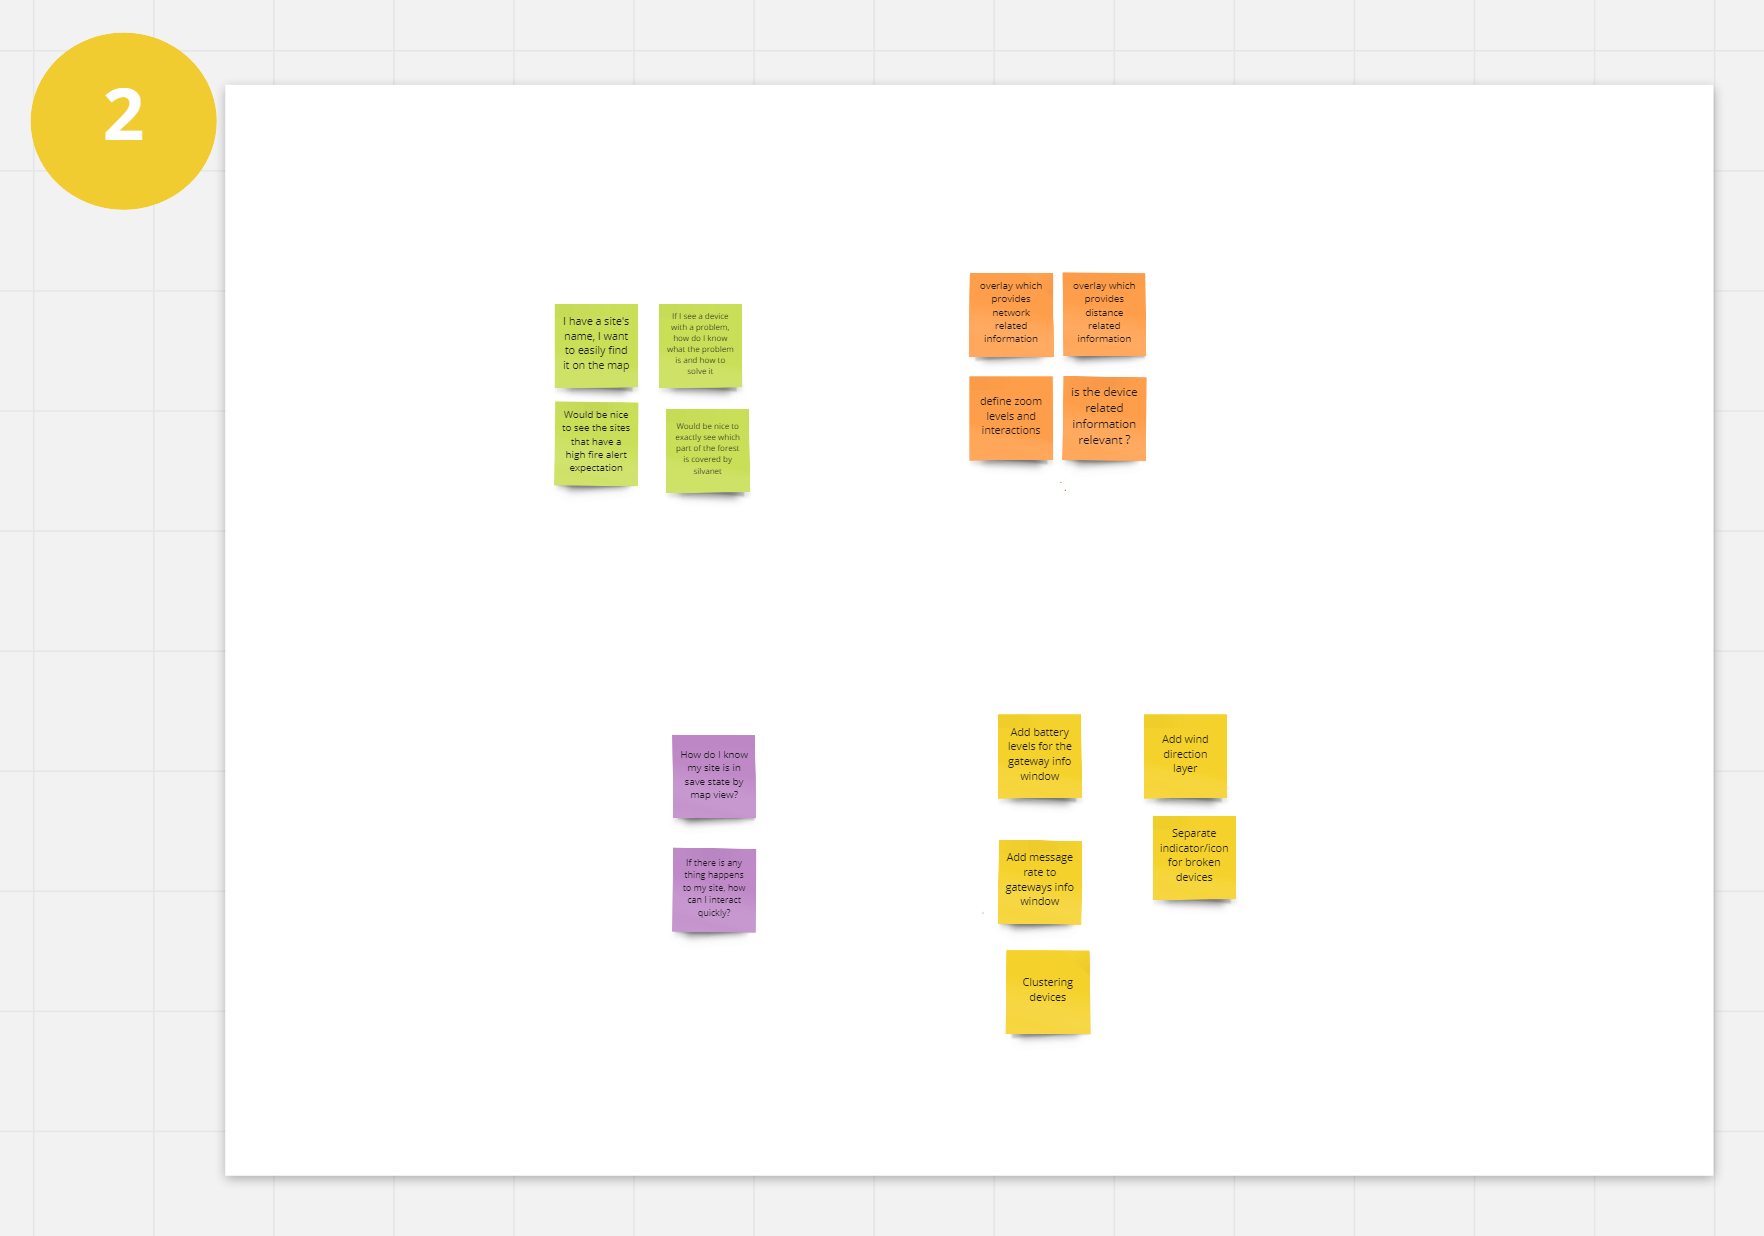
\includegraphics[width=\textwidth]{question_board_map_2}
  \caption{Relevante lose Idee für eine interaktive Karte}
  \label{fig:question_board_map_2}
\end{figure}
\begin{figure}[H]
  \centering
  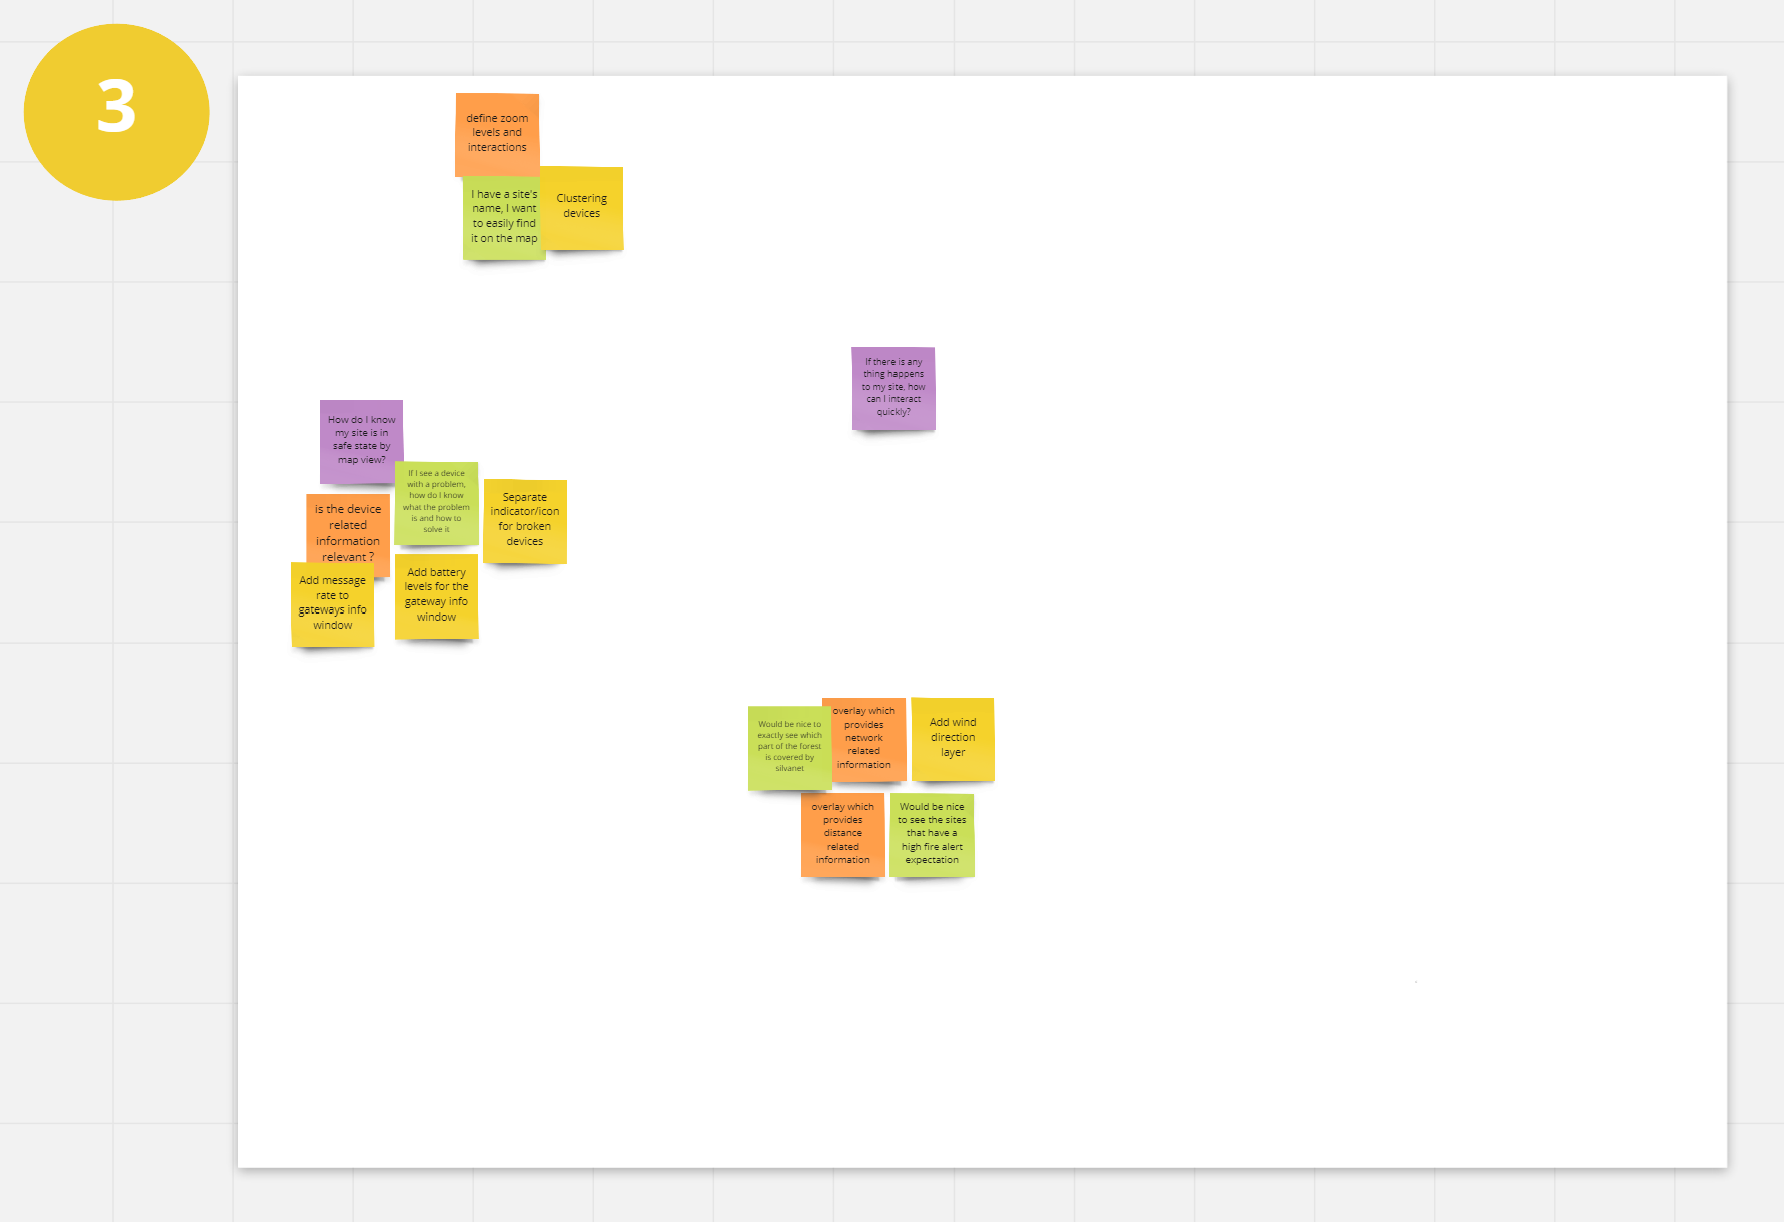
\includegraphics[width=\textwidth]{question_board_map_3}
  \caption{Bündelung von Ideen zu einem gemeinsamen Thema}
  \label{fig:question_board_map_3}
\end{figure}

\section{Nutzerpfad, um den Einsatz eines Sensors zu planen.} \label{appendix:planing_devices_flow}

\begin{figure}[H]
  \centering
  \includegraphics[width=\textwidth]{app_planning_creation_start}
  \caption{Planungsseite bei der Ankunft des Nutzers}
  \label{fig:app_planning_creation_start}
\end{figure}
\begin{figure}[H]
  \centering
  \includegraphics[width=\textwidth]{app_planning_creation_devices}
  \caption{Planungsseite nach dem Hinzufügen eines Sensors}
  \label{fig:app_planning_creation_devices}
\end{figure}
\begin{figure}[H]
  \centering
  \includegraphics[width=\textwidth]{app_planning_creation_device_select}
  \caption{Planungsseite nach Auswahl eines Sensors aus der Liste}
  \label{fig:app_planning_creation_device_select}
\end{figure}

\section{Nutzerpfad, um den Einsatz eines Sensors zu planen mit kognitivem Tunneldesign} \label{appendix:planing_devices_flow_tunneling}

\begin{figure}[H]
  \centering
  \includegraphics[width=\textwidth]{app_planning_creation_v2_name}
  \caption{Planungsseite im Tunneldesign bei der Ankunft des Nutzers}
  \label{fig:app_planning_creation_v2_name}
\end{figure}
\begin{figure}[H]
  \centering
  \includegraphics[width=\textwidth]{app_planning_creation_v2_devices}
  \caption{Planungsseite im Tunneldesign beim Schritt Geräte hinzufügen}
  \label{fig:app_planning_creation_v2_devices}
\end{figure}
\begin{figure}[H]
  \centering
  \includegraphics[width=\textwidth]{app_planning_creation_v2_devices_list}
  \caption{Planungsseite im Tunneldesign nach dem Hinzufügen von Geräten }
  \label{fig:app_planning_creation_v2_devices_list}
\end{figure}
\begin{figure}[H]
  \centering
  \includegraphics[width=\textwidth]{app_planning_creation_v2_device_selected}
  \caption{Planungsseite im Tunneldesign bei der Auswahl eines Geräts}
  \label{fig:app_planning_creation_v2_device_selected}
\end{figure}
\begin{figure}[H]
  \centering
  \includegraphics[width=\textwidth]{app_planning_creation_v2_add_more}
  \caption{Planungsseite im Tunneldesign mit Geräteliste und Auswahlfeldern zum Hinzufügen weiterer Geräte}
  \label{fig:app_planning_creation_v2_add_more}
\end{figure}

\begin{figure}[H]
  \centering
  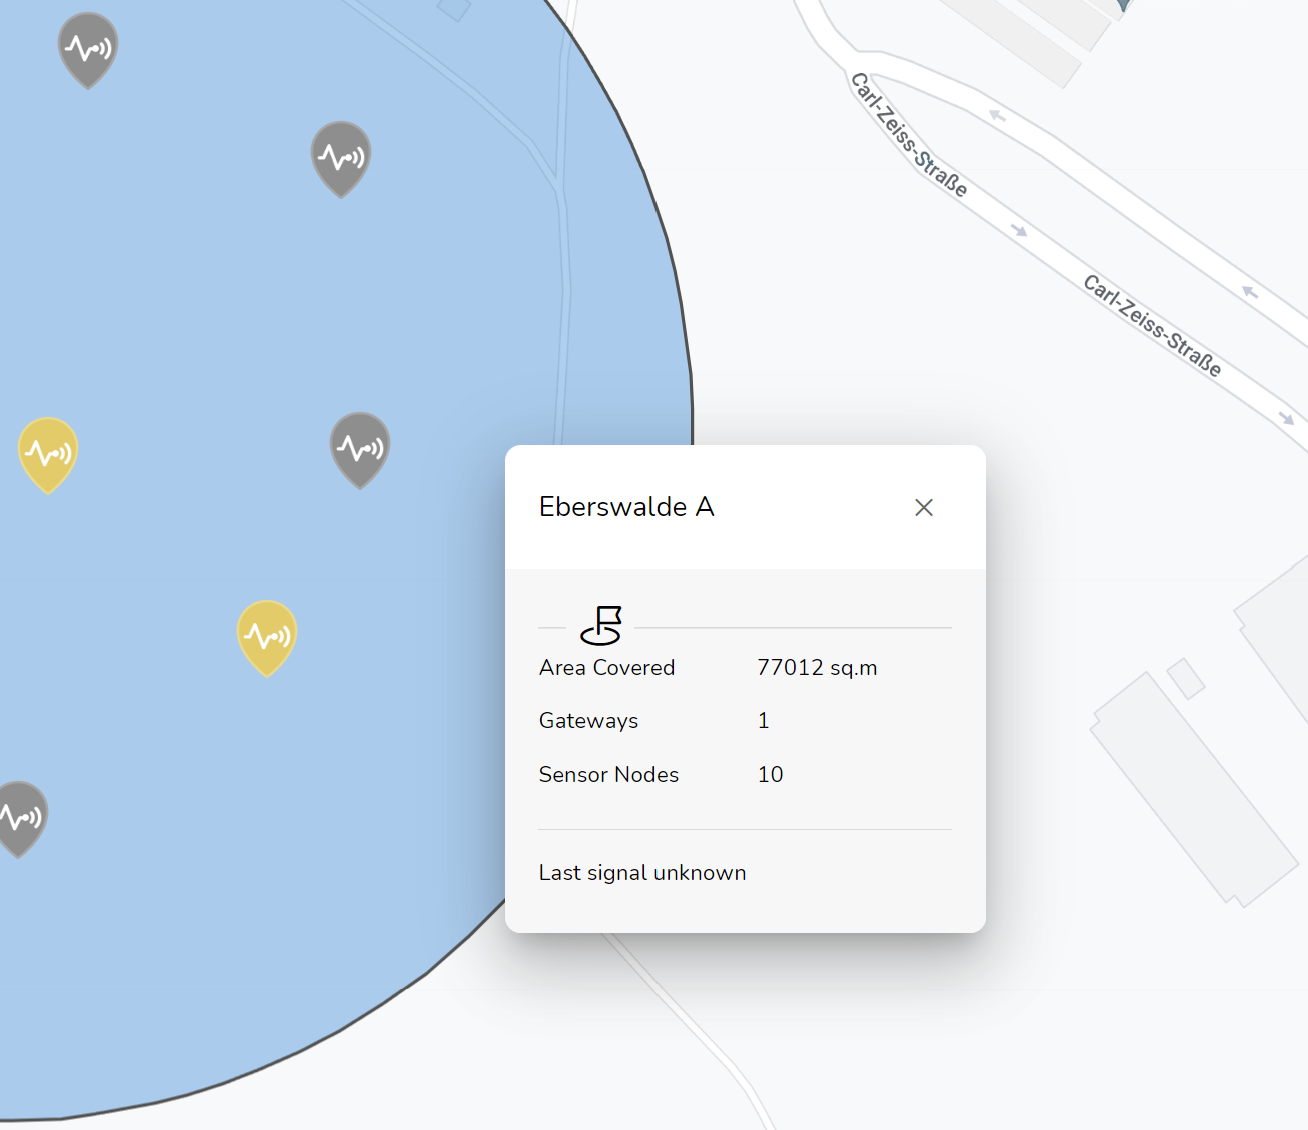
\includegraphics[width=8cm]{map_old_site_details}
  \caption{Anzeige der Details einer \textit{Site} auf der ursprünglichen interaktiven Karte}
  \label{fig:map_old_site_details}
\end{figure}

\section{Prototyping des Zoomverhaltens der interaktiven Karte} \label{appendix:map_flow}

\begin{figure}[H]
  \centering
  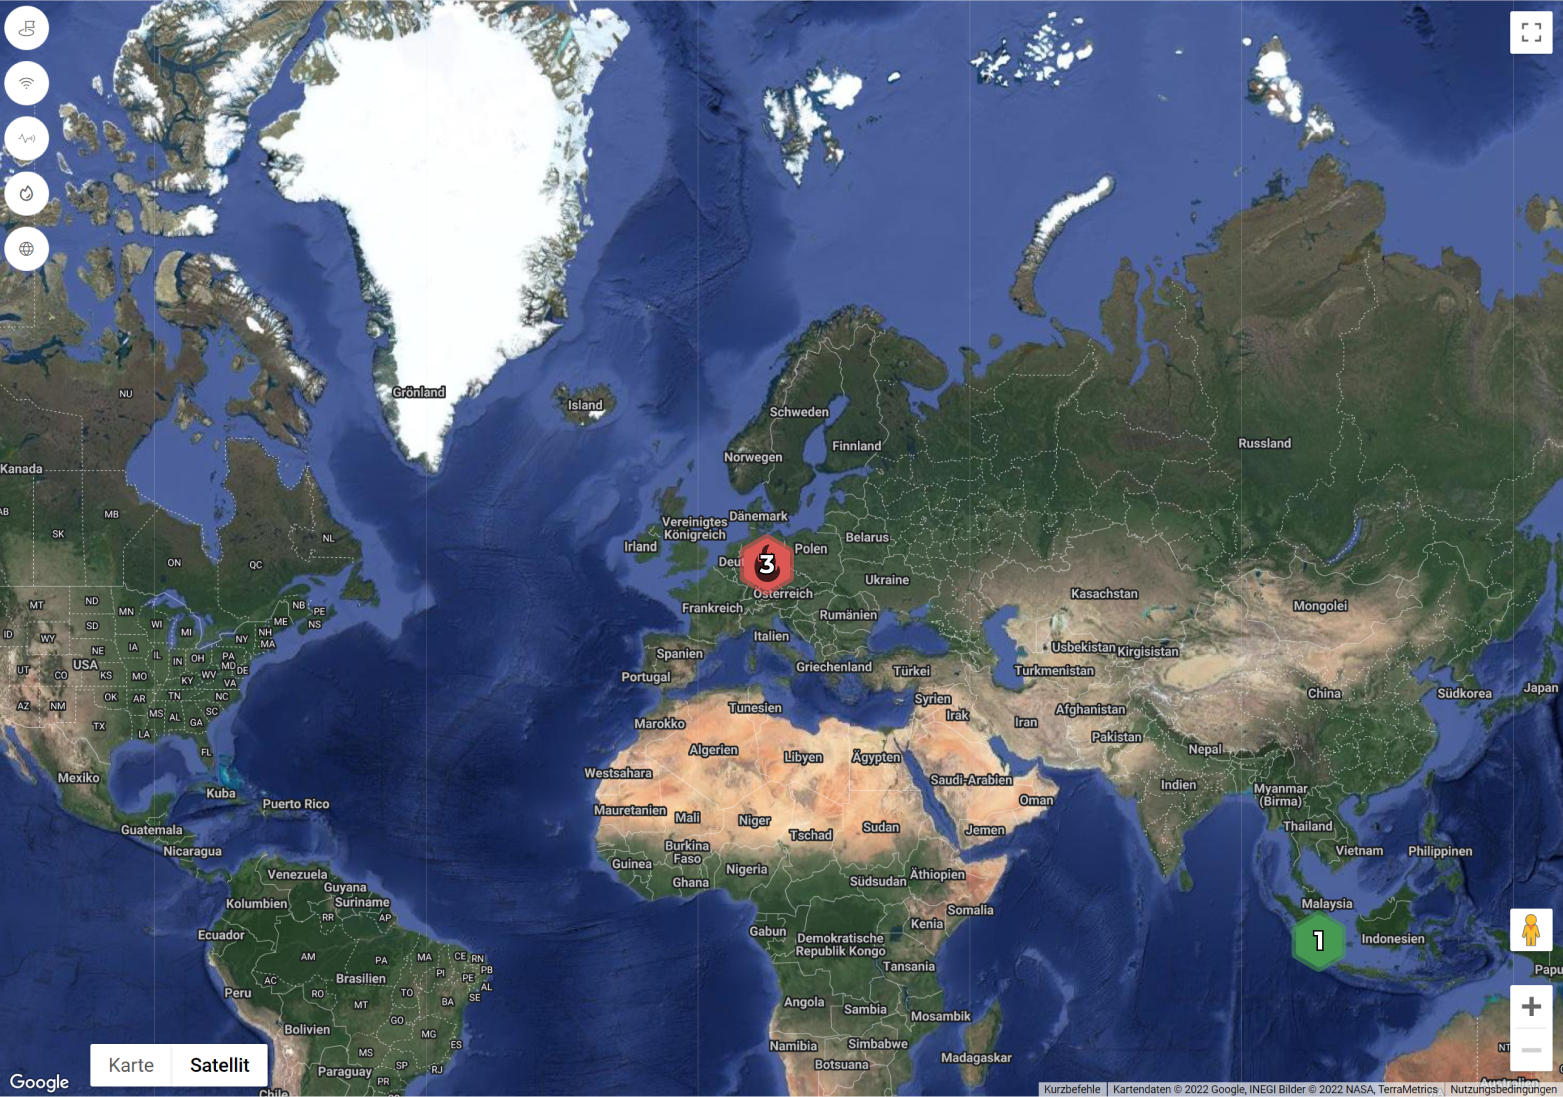
\includegraphics[width=10cm]{map_clustering_level-1}
  \caption{Interaktive Karte in Zoomstufe 1}
  \label{fig:map_clustering_level-1}
\end{figure}
\begin{figure}[H]
  \centering
  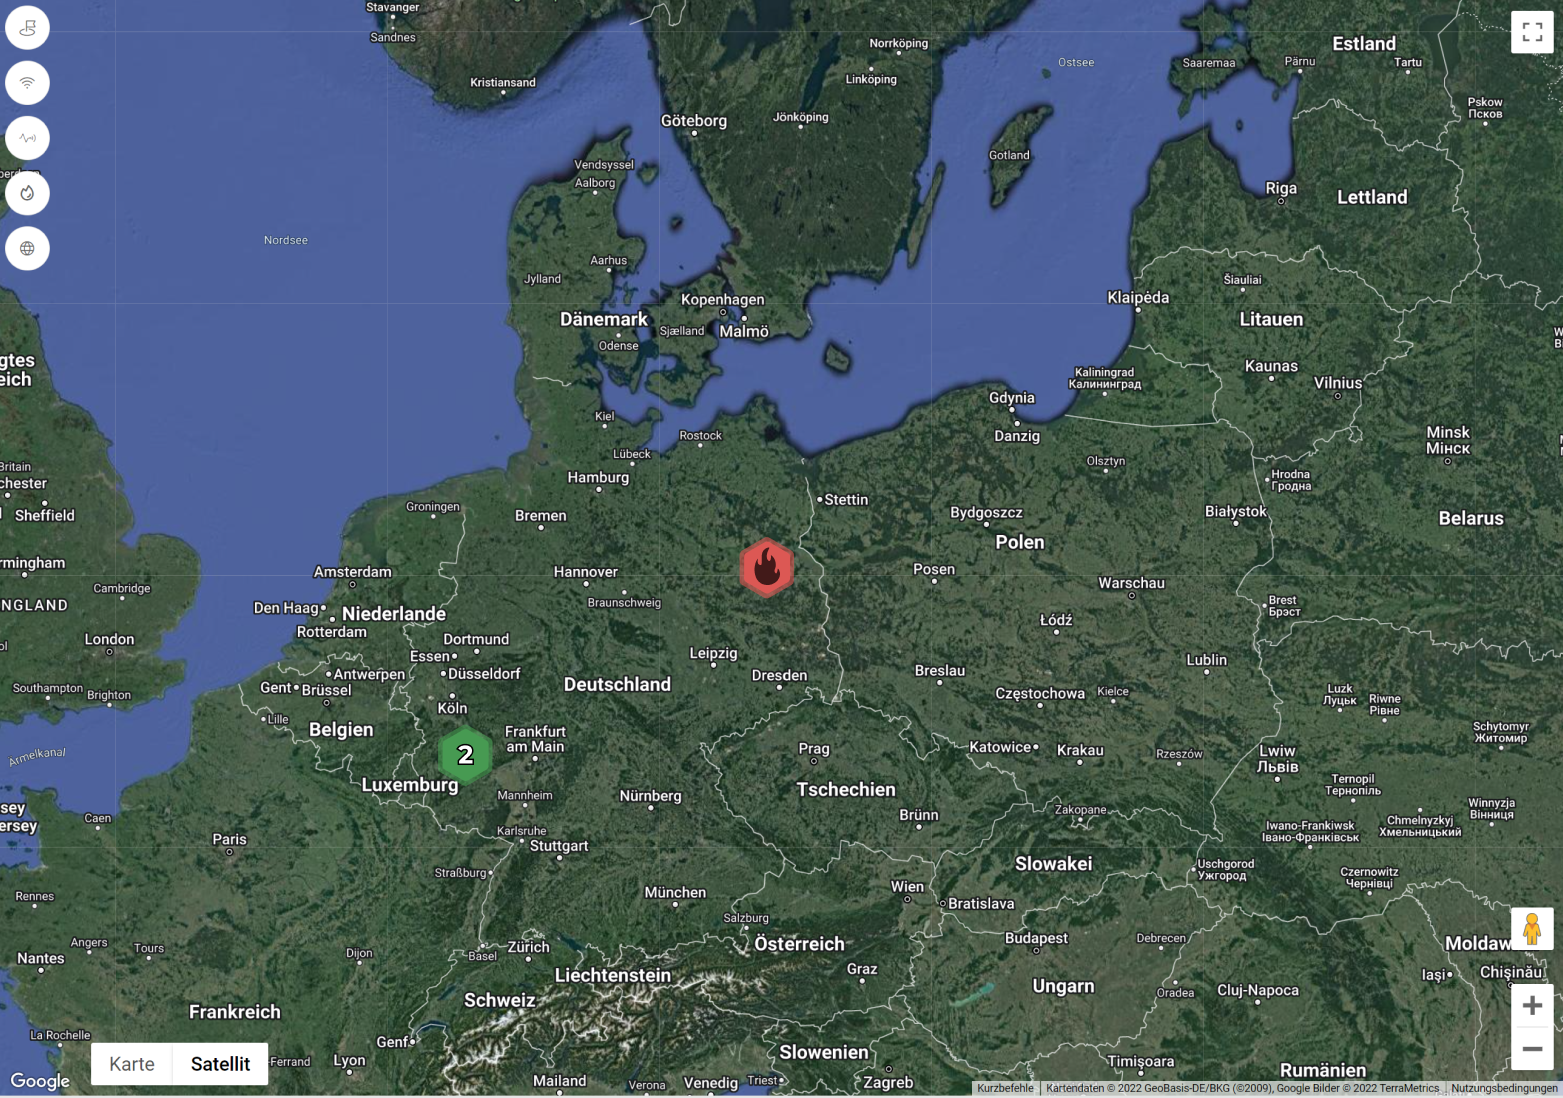
\includegraphics[width=10cm]{map_clustering_level-6}
  \caption{Interaktive Karte in Zoomstufe 6}
  \label{fig:map_clustering_level-6}
\end{figure}
\begin{figure}[H]
  \centering
  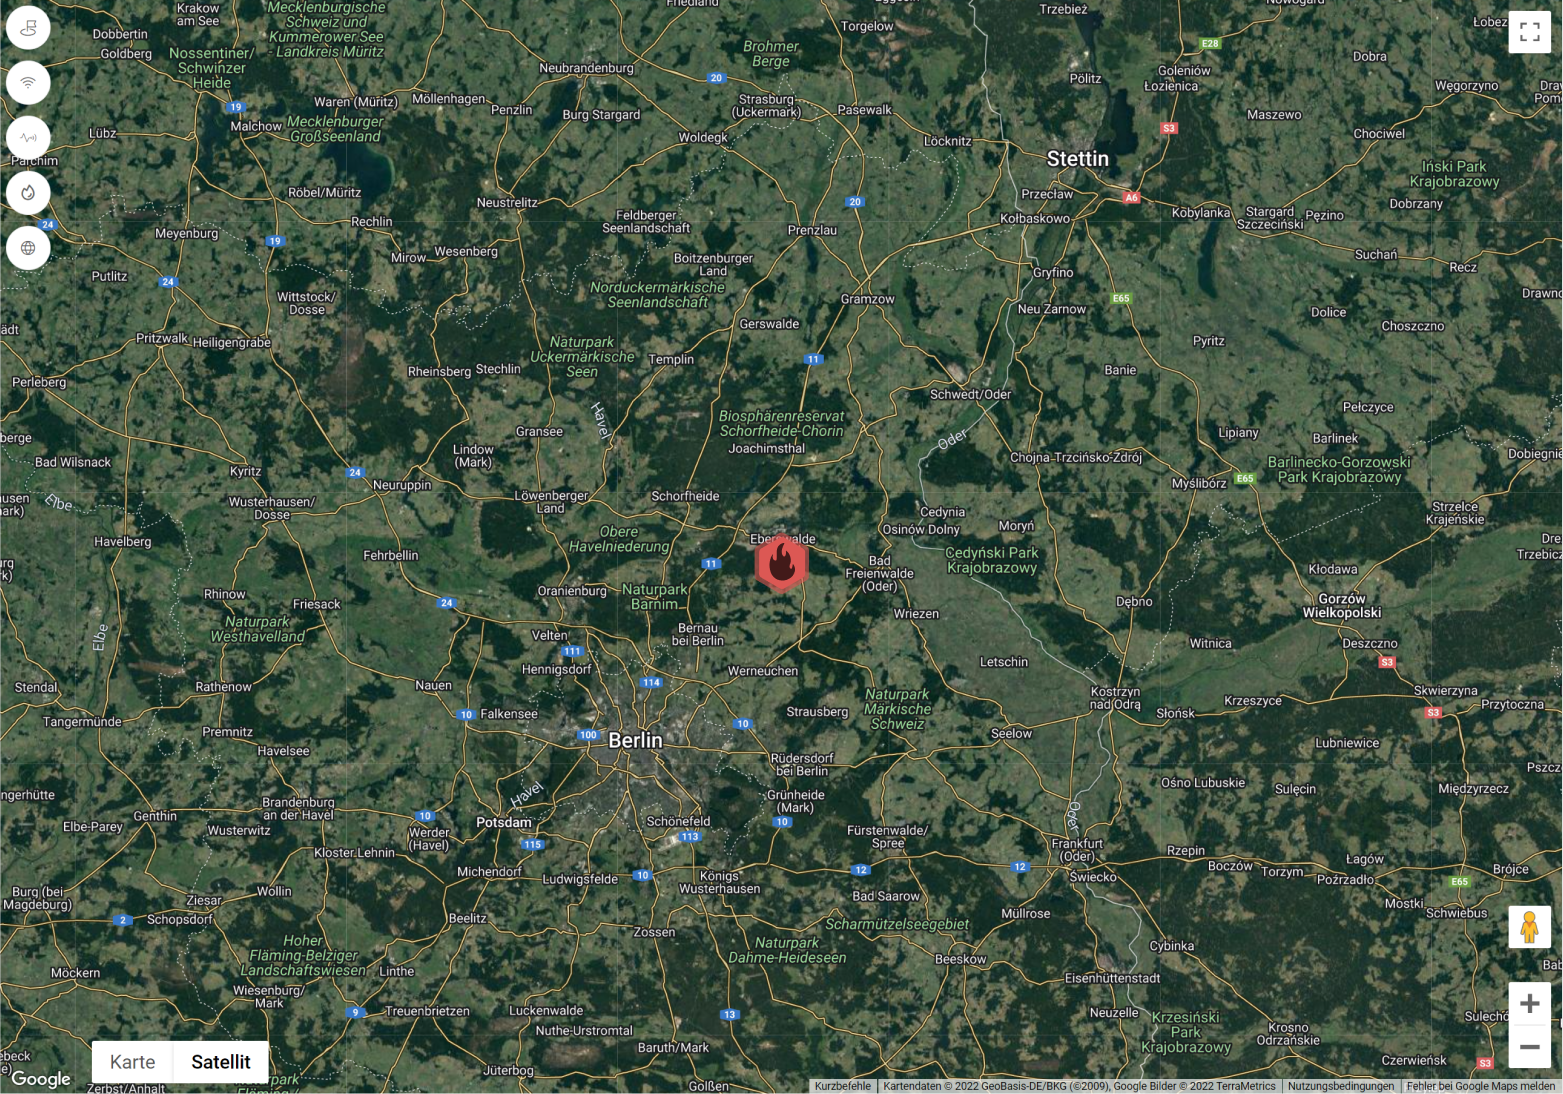
\includegraphics[width=10cm]{map_clustering_level-9}
  \caption{Interaktive Karte in Zoomstufe 9}
  \label{fig:map_clustering_level-9}
\end{figure}
\begin{figure}[H]
  \centering
  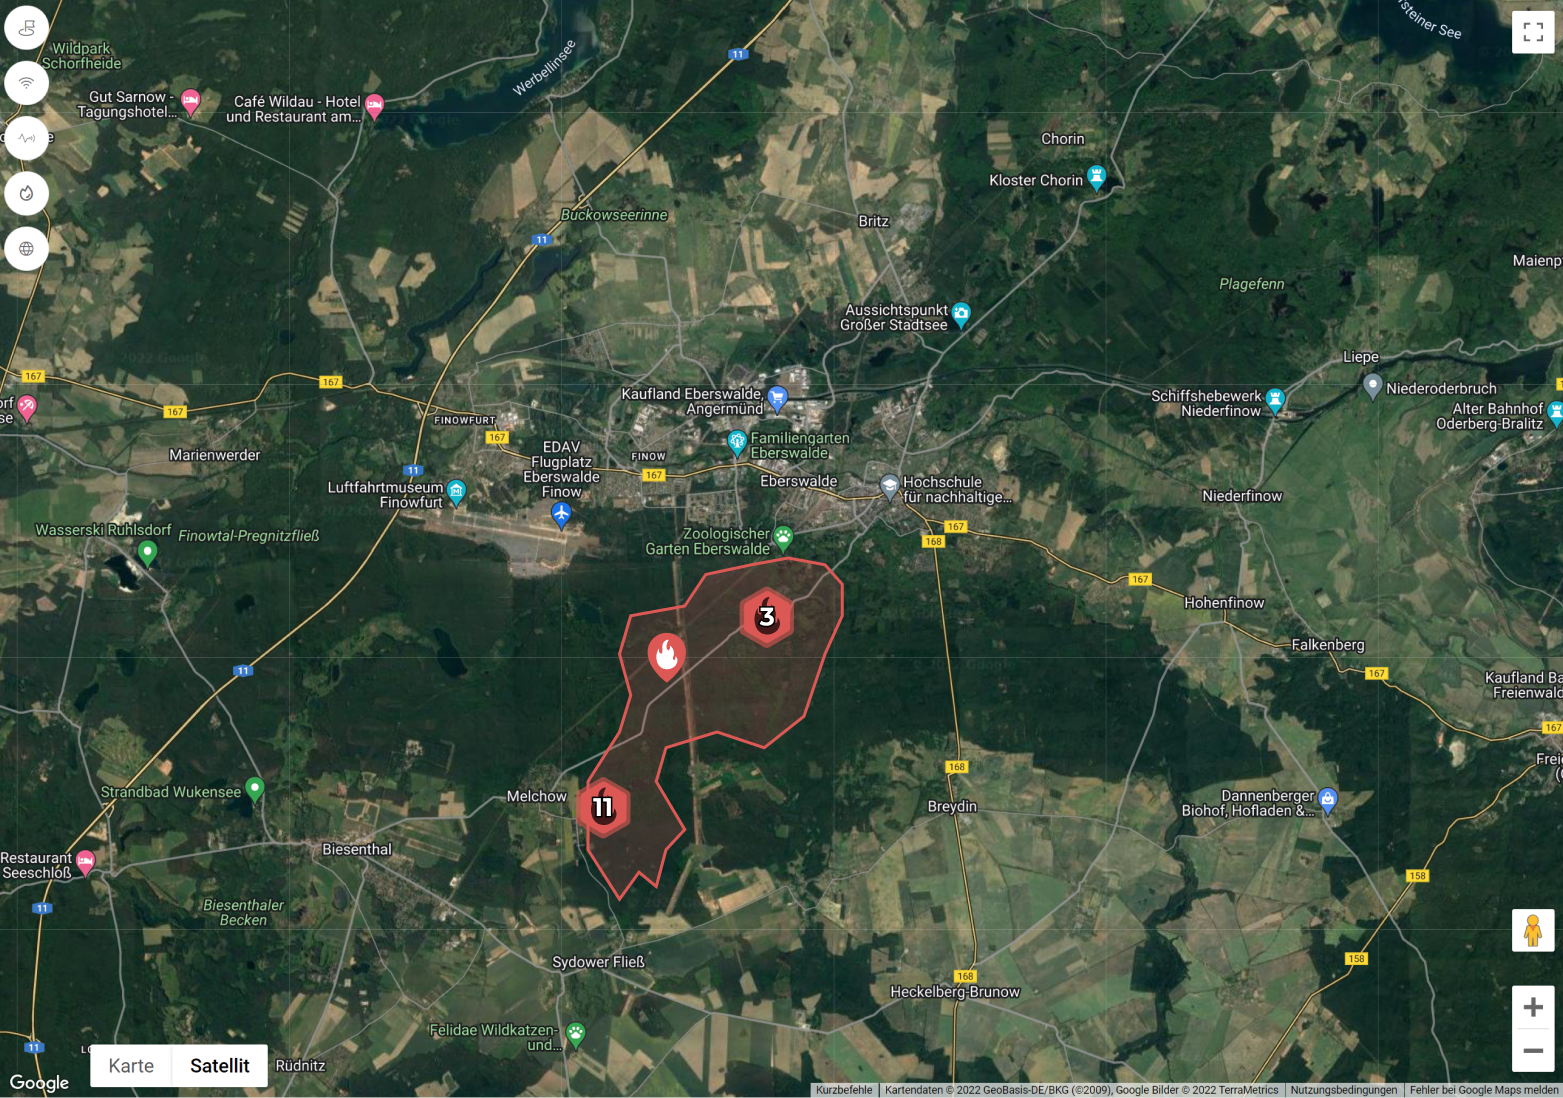
\includegraphics[width=10cm]{map_clustering_level-12}
  \caption{Interaktive Karte in Zoomstufe 12}
  \label{fig:map_clustering_level-12}
\end{figure}
\begin{figure}[H]
  \centering
  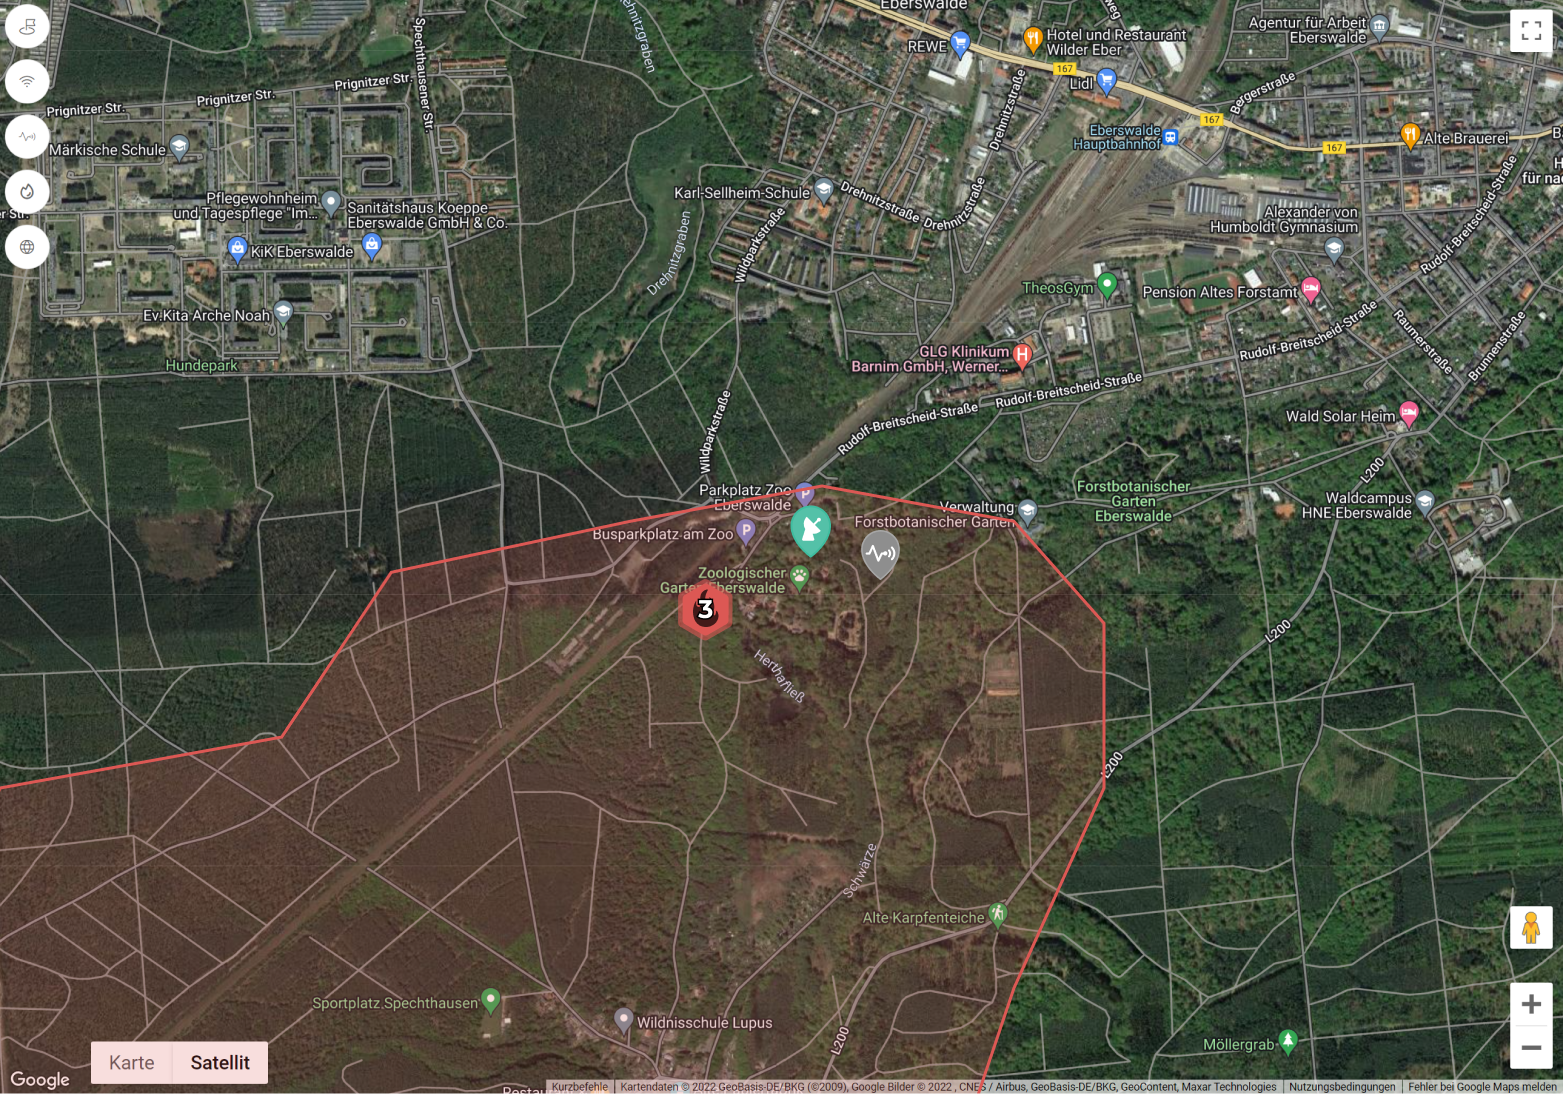
\includegraphics[width=10cm]{map_clustering_level-14}
  \caption{Interaktive Karte in Zoomstufe 14}
  \label{fig:map_clustering_level-14}
\end{figure}
\begin{figure}[H]
  \centering
  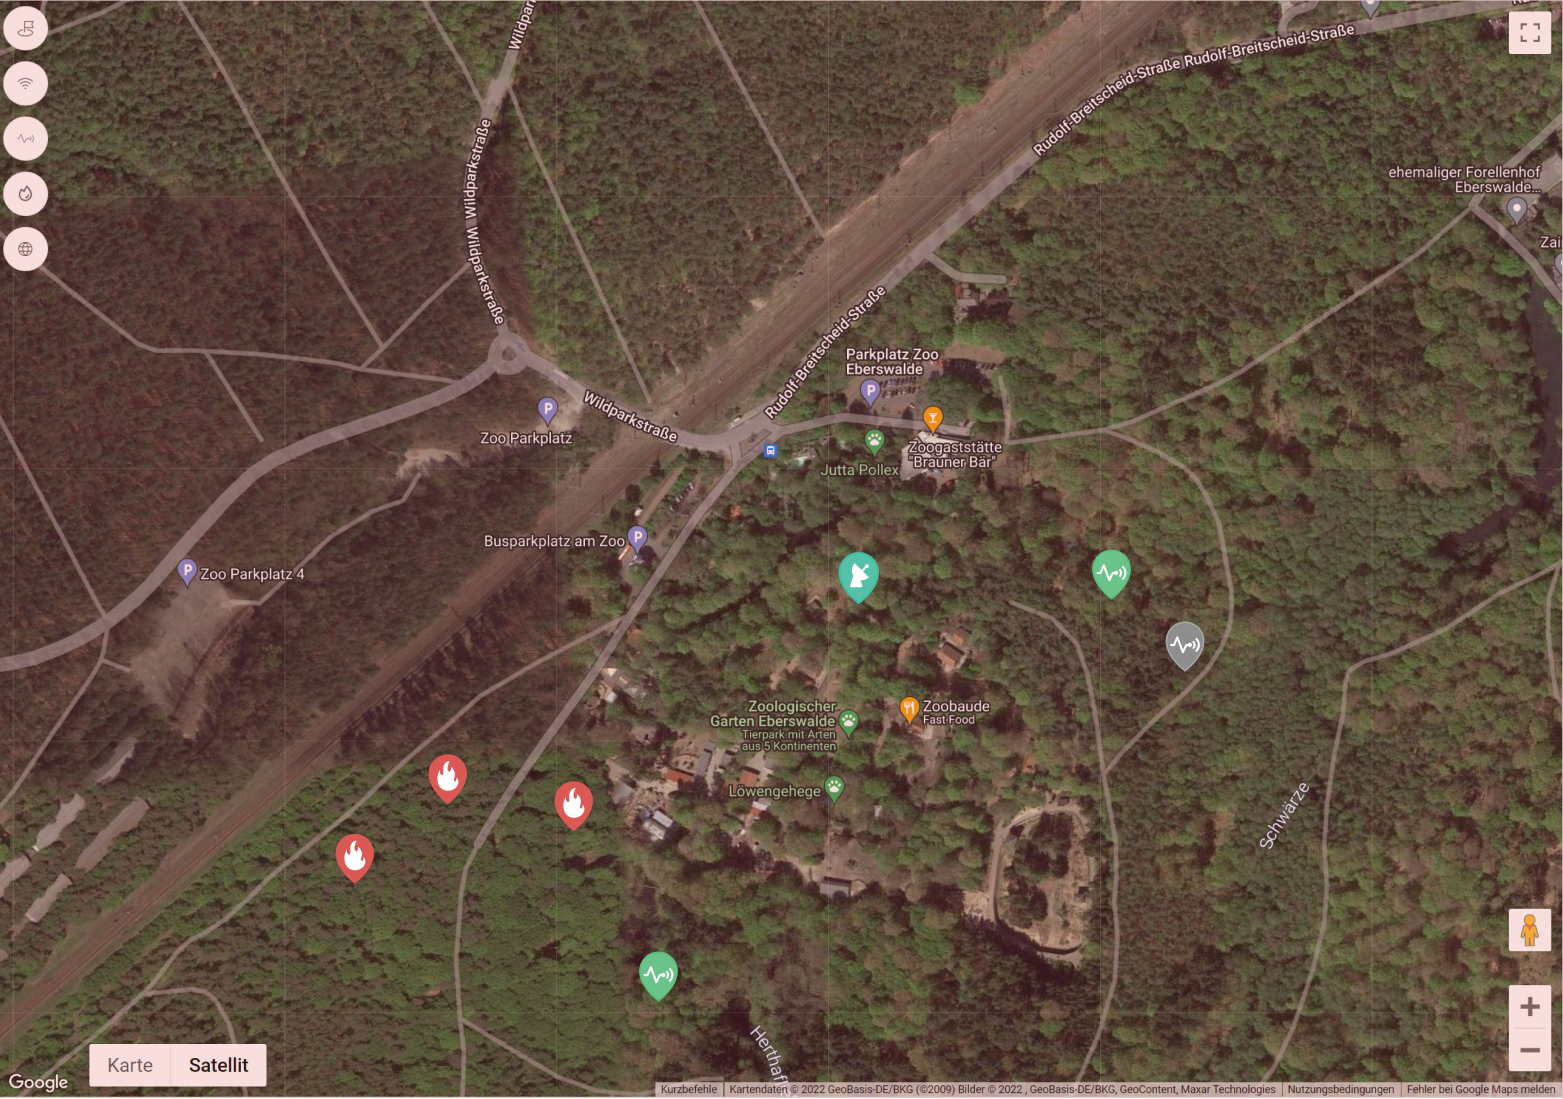
\includegraphics[width=10cm]{map_clustering_level-17}
  \caption{Interaktive Karte in Zoomstufe 17}
  \label{fig:map_clustering_level-17}
\end{figure}


\begin{lstlisting}[
  language=javascript,
  caption={Vereinfachter Code für die \lstinline{getUrlPortionLabel}-Methode},
  captionpos=b,
  label={lst:getUrlPortionLabel}
]
const capitalizeFirstLetter = (chars: string): string => {
  return chars.charAt(0).toUpperCase() + chars.slice(1);
}

private getUrlPortionLabel = (urlPortion: string): string => {
  const isNumber = !isNaN(urlPortion)

  if (!isNumber) {
    const isAction = urlPortion.startsWith("_")
    if (isAction) urlPortion = urlPortion.slice(1) // remove first char in string

    return capitalizeFirstLetter(urlPortion)
  }

  return urlPortion
}
\end{lstlisting}

\section{Unterzeichnung der API, die für die interaktive Karte gedacht ist} \label{appendix:map-api}
\subsection{Liste der \textit{Sites}}

\textbf{GET /sites/status}

Die Antwort ist ein Array aus Elementen vom Typ \lstinline{SiteStatus}:

\begin{lstlisting}[
  language=javascript,
  caption={TypeScript Interface vom Typ \lstinline{SiteStatus}},
  captionpos=b
]
interface SiteStatus {
  id: number
  name: string
  centerLatitude: number
  centerLongitude: number
  fireAlertStatus: number // 1: maybe fire; 2: fire detected
  lastMessageTimestamp: string // used to detect bad connectivity
  batteryLevel: number // used to detect bad sun exposition
}
\end{lstlisting}

\subsection{Liste der Sensoren eines \textit{Site}}

\textbf{GET /sites/:siteId/sensornodes/status}

Die Antwort ist ein Array aus Elementen vom Typ \lstinline{SensorNodeStatus}:

\begin{lstlisting}[
  language=javascript,
  caption={TypeScript Interface vom Typ \lstinline{SensorNodeStatus}},
  captionpos=b
]
interface SensorNodeStatus {
  id: number
  name: string
  latitude: number
  longitude: number
  fireAlertStatus: number
  lastMessageTimestamp: string
  batteryLevel: number
}
\end{lstlisting}

\begin{lstlisting}[
  language=javascript,
  caption={TypeScript Interface vom GeoJSON-Punkteigenschaften von \textit{Sites} und Sensoren},
  captionpos=b,
  label={lst:pointsproperties}
]
interface SiteProperties {
  site_id: string
  name: string
  lat: number
  lng: number
  fire_alert?: AlertPhases // 1 or 2
  offline?: boolean
  maintenance?: boolean
}

type DeviceProperties = Omit<SiteProperties, "site_id"> & { id: number; type: "sensor" | "gateway" }
\end{lstlisting}